% !TeX root = ../main.tex
% Add the above to each chapter to make compiling the PDF easier in some editors.

\chapter{Grundlagen}\label{chapter:Literaturrecherche}
Dieses Kapitel stellt die Ergebnisse einer umfassenden Literaturrecherche dar. Zunächst wird auf Definitionen eingegangen, die für die Unfallforschung relevant sind. Darauf folgt ein Überblick über Unfallzahlen in Deutschland innerhalb geschlossener Ortschaften. Des weiteren werden urbane Fahrsituationen hinsichtlich ihrer Komplexität und möglichen Konfliktpunkten genauer betrachtet. Im Verlauf der Arbeit soll eine Bewertungsskala für urbane Fahrsituationen erstellt werden, weshalb am Ende des Kapitels bereits vorhandene Skalen zur Bewertung vorgestellt werden. Der Übersichtlichkeit halber sind unter dem Begriff Fahrer bzw. Fahrzeugführer sowohl Fahrer als auch Fahrerinnen zu verstehen. Gleiches gilt für Fußgänger/Fußgängerinnen sowie Radfahrer/Radfahrerinnen.

\section{Definitionen und wichtige Begriffe der Unfallforschung}
Dieses Kapitel dient dazu Begriffe, die im Verlauf dieser Arbeit häufig genannt werden, zu erläutern. Im Fokus stehen vor allem  Begriffe, die in der Unfallforschung und bei der polizeilichen Unfallaufnahme eine Rolle spielen.

%Evtl. noch Personenschaden vs. Verunglückte hinzufügen.

\subsection{Risiko}
Der Begriff Risiko wird im Duden als \enquote{möglicher negativer Ausgang bei einer Unternehmung, mit dem Nachteile, Verlust, Schäden verbunden sind; mit einem Vorhaben, Unternehmen o.Ä. verbundenes Wagnis} definiert. Im Straßenverkehr wird das Risiko häufig etwas konkreter als das Produkt von Auftretenswahrscheinlichkeiten und Gefahr angegeben. Die Gefahr kann anhand der Verletzungsschwere \parencite[S. 151f.]{Huguenin.2017} oder Schadenhöhe \parencite[S. 60]{Gschwendtner.2015} angegeben werden. Das Grenzrisiko stellt dabei \enquote{das größte noch vertretbare Risiko eines bestimmten technischen Vorgangs oder Zustands} dar \parencite[S. 43]{Hillenbrand.2012}.

Der Begriff Risiko und dessen Wahrnehmung kann in drei verschiedene Richtungen interpretiert werden. Hierbei entspricht das \enquote{Objektive (statische) Risiko} der Wahrscheinlichkeit in einen Unfall verwickelt zu sein, das \enquote{Subjektive Risiko} gibt an, wie der Fahrer es selbst abschätzt in einen Unfall verwickelt zu werden und das \enquote{Gefühlte Risiko} gibt Auskunft darüber, wie der Fahrer die Bedrohlichkeit emotional beurteilt \parencite[S. 461f]{Fuller.2005}.

\subsection{Gefahr}
Gefahr beschreibt einen Zustand oder Vorgang aus dem ein Schaden für Personen und/oder Sachgüter zwangsläufig oder zufällig entsteht, ohne das ausreichende Gegenmaßnahmen gewährleistet sind. \enquote{Der Begriff bezeichnet eine Bedrohung durch ein zukünftiges Schadensereignis, das unter bestimmten Bedingungen eintreten kann} \parencite[S. 8]{Hoffmann.26.04.2013}. Gefahr kann auch als Sachlage, bei der das Risiko größer als das Grenzrisiko ist verstanden werden. Die Gefährdung hingegen beschreibt eine Situation, in der eine tatsächliche oder mögliche Gefahr für Personen oder die Umwelt eines betrachteten Systems besteht \parencite[S. 43f]{Hillenbrand.2012}.

\subsection{Sicherheit}
Nach \Textcite[S. 40]{Fricke.2006} wird das Maß an Sicherheit beschrieben als das Risiko, unerwünschte Konsequenzen materiellen oder personellen Schaden zu erleiden. Unter dem Begriff Risiko ist in diesem Zusammenhang die Wahrscheinlichkeit zu verstehen, dass sich ein potentiell gefährlicher Zustand einstellt, bzw. sich eine potentiell gefährliche Situation ergibt. Häufig wird Sicherheit auch durch Gleichungen beschrieben:

\begin{itemize}
	\item Sicherheit = 1 - Unfallwahrscheinlichkeit \parencite[S. 24]{Hoffmann.26.04.2013}
	\item Sicherheit = 1 - Gefahr \parencite[S. 42]{Hillenbrand.2012}
\end{itemize}

Zusammenfassend kann Sicherheit als das Nichtvorhandensein einer Gefahr für Menschen oder Sachwerte verstanden werden \parencite[S. 42]{Hillenbrand.2012}. Es kann zwischen Betriebssicherheit (Schutz der Umgebung vor einer Sache) und Angriffssicherheit (Schutz einer Sache vor der Umgebung) unterschieden werden. Betrachtet man den Verkehrsbereich geht man Häufig von Betriebssicherheit aus. Ein Beispiel hierfür wäre, dass die Fußgänger oder Radfahrer, in der Umgebung eines Kfz, besonders Schutzbedürftig bei einer Kollision mit diesem sind. 

Bei dem Begriff der Verkehrssicherheit wird oft vom Kontinuum des Verkehrsverhaltens vom Normalverhalten bis zum Unfall ausgegangen \parencite[S. 9]{Hoffmann.26.04.2013}. Wenn man von der Sicherheit einer gewissen Einheit im Verkehrswesen, z.B. einer bestimmten Kreuzung, spricht kann die Sicherheit der Einheit durch die Anzahl der Unfälle die in einer spezifischen Zeitspanne auftreten beschrieben werden. Es wird nicht nur die Anzahl der Unfälle gezählt, sondern auch aufgenommen um was für einen Unfalltyp oder Unfallart es sich handelt und was der Unfall für Folgen hatte \parencite[S. 3]{Antoniou.21.06.2018}.

\enquote{Im Bereich der Fahrzeugsicherheit wird mit dem Begriff \enquote{Sicherheit} eine Situation beschrieben, bei der das erzielbare Risiko kleiner ist als das größte noch vertretbare Risiko (Grenzrisiko) eines bestimmten technischen Vorgangs oder Zustands. Je größer aber das Risiko ist, desto geringer ist die Sicherheit, und umgekehrt gilt, je höher die Sicherheit gesteigert werden soll, desto geringer darf das Risiko nur sein} \parencite[S. 743]{Burg.2017}. Bei dem Begriff der Sicherheit kann zwischen aktiv und passiv unterschieden werden. Während aktive Maßnahmen, Maßnahmen darstellen, die Unfälle vermeiden, werden unter passiver Sicherheit Maßnahmen verstanden, die die Unfallfolgen mindern. Obwohl durch eine Verbesserung der aktiven Sicherheit die Anzahl der Unfälle reduziert werden kann kam es in den letzten Jahren, im Bereich der Fahrzeugsicherheit, überwiegend zu Neuerungen der passiven Sicherheit.

Bei aktuellen Entwicklungen im Bereich der \ac{FAS} wird der Fokus vermehrt auf aktive Maßnahmen gelegt. Zu den aktiven Maßnahmen gehören jedoch nicht nur Neuerungen am Fahrzeug und unterstützende Systeme, sondern auch die entsprechende Schulung der Verkehrsteilnehmer z.B. mit Fahrsicherheitstrainings oder eine entsprechende Gestaltung der Verkehrswege um Unfallschwerpunkte zu vermeiden.

Häufig wird auch der Begriff der Sicherheitsrelevanz verwendet. \enquote{Als sicherheitsrelevant werden Systeme bezeichnet, die entweder selbst Gefahren verursachen können, oder aber für die Reduzierung von Risiken eingesetzt werden} \parencite[S. 44]{Hillenbrand.2012}. Als sicherheitskritisch werden dahingegen technische Systeme beschrieben, \enquote{bei welchen Aktuatoren von Kontrolleinheiten angesteuert werden. Durch die Tatsache, dass Aktuatoren die Bedienungen der physikalischen Umgebung verändern können, besteht die Möglichkeit der Gefahr für Leib und Leben} \parencite[S. 44]{Hillenbrand.2012}. Eine Situation wird also kritisch, wenn sie zu Verletzungen führen kann.

\Textcite[S. 10]{Hoffmann.26.04.2013} stellt fest, dass die Grenzen  zwischen \enquote{sicher} und \enquote{unsicher} fließend, subjektiv und variabel sind. In Abbildung \ref{fig:sicher_unsicher} wird der Übergang einer sicheren Situation in eine Unsichere, die zum Unfallführen kann dargestellt. Zusätzlich ist zu erkennen, dass mit höherem Risiko die Sicherheit abnimmt. 

\begin{savenotes}
	\begin{figure}[H]
		\centering
		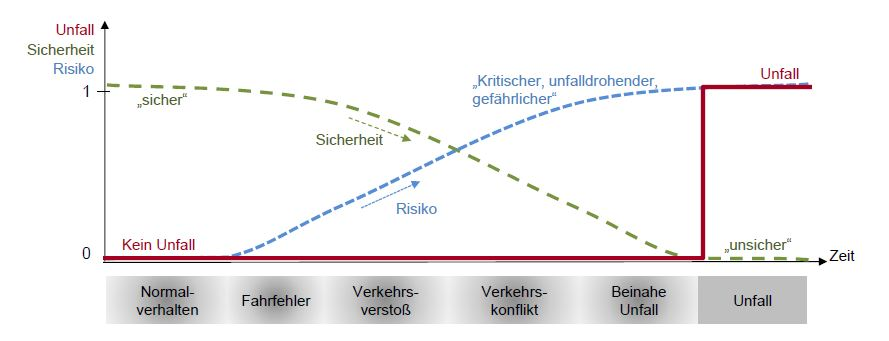
\includegraphics[width=14cm,height=6cm]{figures/sicher_unsicher}
		\caption[Darstellung zur Beschreibung von Verkehrssicherheit und -unsicherheit]{Darstellung zur Beschreibung von Verkehrssicherheit und -unsicherheit \parencite[S. 10]{Hoffmann.26.04.2013}}\label{fig:sicher_unsicher}
	\end{figure}
\end{savenotes}

\subsection{Verkehrssituation}
Laut \Textcite[S. 6-8]{Hoffmann.26.04.2013} gibt es keine allgemeingültige Definition für den Situationsbegriff im verkehrswissenschaftlichen Zusammenhang. Dies gilt auch für die Grenze zwischen zwei Situationen. Es wird häufig zwischen objektiv gegebenen Situationen und subjektiv wahrgenommenen Teilen einer Situation unterschieden. Der Unterschied der beiden Situationen kann das Verhalten der Verkehrsteilnehmer stark beeinflussen.

\Textcite[S.43]{Reichart.2001} gibt verschiedene Perspektiven auf Situationen im Straßenverkehr an. Neben der Verkehrssituation unterscheidet er zwischen Fahrsituation und Fahrersituation. Unter dem Begriff \enquote{Verkehrssituation} versteht man die objektiv gegebene räumliche und zeitliche Konstellation der verkehrsbezogenen Einflussgrößen der Umgebung aus der Perspektive des Verkehrsteilnehmers. Hierunter sind z.B. Umfeldgegebenheiten, wie die Art der Verkehrsregelung, die Gestaltung der Fahrbahn oder die Art des Knotenpunktes zu verstehen. Die \enquote{Fahrsituation} beschreibt den aus Fahrersicht prinzipiell wahrnehmbaren Ausschnitt der Verkehrssituation in Abhängigkeit des geplanten Fahrmanövers und des umgebenden Verkehrs. Auch in dieser Situation wird die Umgebungsgestaltung rein objektiv beschrieben. Neben der Berücksichtigung anderer Verkehrsteilnehmer wird hier auch die Vorfahrtssituation (Wartepflichtig oder Vorfahrtsberechtigt) betrachtet. Unter der \enquote{Fahrersituation} ist die tatsächlich vom Fahrer wahrgenommene Sichtweise auf die Fahr- und Verkehrssituation zu verstehen. Die Art der Fahrersituation wird stark von den momentanen physischen und psychischen Eigenschaften des Fahrers bestimmt. Im Hinblick auf die folgende Auswertung der Unfalldaten sind vor allem die Begriffe Verkehrssituation und Fahrsituation wichtig. Sie können bei der Einordnung und Klassifizierung der verschiedenen Unfällen hilfreich sein. Die vorliegenden Daten geben leider keine Auskunft über bestimmte Eigenschaften des Fahrers vor dem Unfall, es ist z.B. nicht bekannt ob er durch die Nutzung eines Handys abgelenkt war. Deshalb wird auf diese Situation im Folgenden nicht näher eingegangen.

\subsubsection{Kritische Verkehrssituationen}
\enquote{Eine kritische Verkehrssituation ist eine Verkehrssituation, bei der ein Eingreifen notwendig wird um die Gefahr eines Verkehrsunfall auszuschließen oder zumindest zu vermindern} \parencite[S. 4]{MockHecker.1994}. Hierbei kann die kritische Situation nicht allein an äußeren Umständen festgemacht werden. Jede normale Fahrsituation kann sich zu einer kritischen Situation entwickeln, wenn der Fahrer sich überfordert oder seine Kompensationsfähigkeit plötzlich überschritten wird \parencite[S. 76]{Bock.1989}. Sobald der Fahrer nicht in der Lage ist alle relevanten Informationen aufzunehmen und bei seinen Entscheidungen zu berücksichtigen kann eine kritische Situation entstehen \parencite[S. 2]{Gerstenberger.17.02.2015}. Um im Vorfeld einschätzen zu können, ob es sich um eine kritische Situation handelt muss man über das Verhalten der anderen Verkehrsteilnehmer Bescheid wissen \parencite[S. 3]{MockHecker.1994}. Ein Beispiel hierfür stellt das Überholen bei Gegenverkehr dar. Wenn bekannt ist, dass das überholende Fahrzeug rechtzeitig wieder einscheren kann ist die Situation unkritisch. Das entgegenkommende Fahrzeug schätzt die Lage je nach Fahrer voraussichtlich unterschiedlich ein. Die Entscheidung, wann es sich um eine kritische Situation handelt hängt also im Endeffekt von der subjektiven Einschätzung der einzelnen Personen ab \parencite[S. 39]{Gerstenberger.17.02.2015}.

Nach \Textcite[S. 30]{Schmidt.2010} ist eine Verkehrssituation immer dann kritisch, wenn es zu einer Kollision zwischen Fahrzeuge und Hindernis kommt oder ein definierter Mindestabstand zwischen Fahrzeug und Hindernis unterschritten wird, ohne dass es zur Kollision kommt. Die Gefährlichkeit einer Verkehrssituation kann durch die Kritikalität beschrieben werden. Die Grundlage zur Beurteilung der Kritikalität stellen meist zeitliche Größen dar \parencite[S. 39]{Gerstenberger.17.02.2015}. Kritische Fahrmanöver sind Bremsen, Beschleunigen und Ausweichen bzw. eine Kombination aus diesen drei Fahrmanövern. Je kürzer die Zeit für ein kritisches Fahrmanöver, desto schwerer der Konflikt \parencite[S. 26]{Erke.1978}.

\subsubsection{Komplexe Verkehrssituationen}
Die Komplexität einer Verkehrssituation kann als Zusammensetzung aus den Anforderungen an die Informationsverarbeitung des Fahrers und den Anforderungen aus der Fahrzeugbedienung beschrieben werden. Bei einer innerstädtischen Kreuzung mit einer Lichtsignalanlage ist die Anforderung an die Informationsverarbeitung gering, während die Anforderung an die Fahrzeugbedienung hoch ist. Handelt es sich dagegen um eine beschilderte Kreuzung sind beide Anforderungen hoch \parencite[S. 36f]{Gerstenberger.17.02.2015}.

\subsection{Verkehrskonflikt/Unfallentstehung}
\enquote{Ein Verkehrskonflikt ist eine Gefahrensituation, in der Verkehrsteilnehmer sich räumlich oder zeitlich so annähern, dass eine erhöhte Kollisionsgefahr besteht} \parencite[S. 26]{Erke.1978}. Das Bedeutet, dass nicht jeder Verkehrskonflikt zwangsweise zu einem Unfall führt. Werden jedoch notwendige Manöver zur Unfallvermeidung nicht oder falsch ausgeführt kommt es zur Kollision \parencite[S. 43]{Fricke.2006}. \enquote{Im Allgemeinen wird bei Verkehrskonflikten von voneinander entgegen gerichteten Verhaltenstendenzen von Verkehrsteilnehmern ausgegangen, die bei Einhaltung der Verkehrsregeln nicht stattfinden würden und die bei Beibehaltung des Verhaltens zu einem Unfall führen} \parencite[S. 10]{Hoffmann.26.04.2013}. Die Wahrscheinlichkeit, dass sich ein Unfall aus einem Verkehrskonflikt ereignet liegt schätzungsweise bei $1\ast 10^{-4}$ \parencite[S. 99]{Reichart.2001}.

Erst wenn ein Verhaltensfehler tatsächlich zu einer Kollision mit einem anderen Verkehrsteilnehmer oder einem Hindernis führt spricht man von einem Verkehrsunfall. Abbildung \ref{fig:Unfallentstehung} zeigt ein Unfallentstehungsmodell. Kommt es zu einem Verkehrskonflikt der nicht erfolgreich bewältigt werden kann führt die zu einem Unfall. Verkehrsunfälle stellen seltene Ereignisse dar und unterliegen wenn man sie statistisch betrachtet einer Poisson-Verteilung \parencite[S. 18]{Grundl.2005}. Das Risiko in einen Unfall verwickelt zu sein ist nach der statistischen Betrachtung für jeden Verkehrsteilnehmer gleich und inhärent. Unfälle sind in der Regel durch mehrere Unfallursachen und Risikofaktoren bedingt und werden durch ein gelegentliches Zusammentreffen dieser Faktoren verursacht \parencite[S. 20]{Grundl.2005}.

\begin{savenotes}
	\begin{figure}[H]
		\centering
		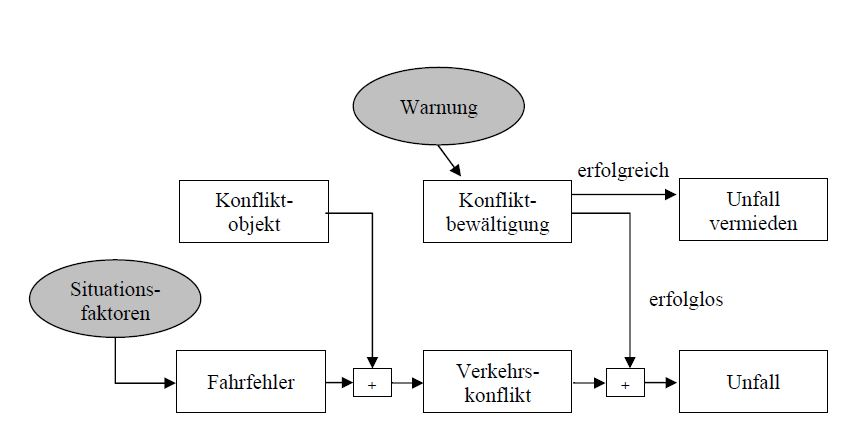
\includegraphics[width=14cm,height=7cm]{figures/Unfallentstehung}
		\caption[Unfallentstehungsmodell]{Unfallentstehungsmodell \parencite[S. 44]{Fricke.2006}}\label{fig:Unfallentstehung}
	\end{figure}
\end{savenotes}

Um den Ablauf eines Verkehrsunfalls zu beschreiben werden oft der Unfalltyp und die Unfallart verwendet. Darüber hinaus ist die Unfallursache ein weiteres wichtiges Klassifizierungsmerkmal, das vor allem in der Unfallforschung genutzt werden kann \parencite[S. 16]{Gschwendtner.2015}. Um Unfälle genau analysieren zu können müssen jedoch viele Einzelursachen und Risikofaktoren betrachtet werden. Bei den Einzelursachen kann z.B. in Haupt- und Mitursachen bzw. direkte oder indirekte Ursachen unterschieden werden. Eine Hauptursache stellt z.B. das Abgelenkt sein dar, als Nebenursache kann z.B. die Eile oder Stimmung des Verkehrsbeteiligten genannt werden \parencite[S. 65-72]{Grundl.2005}. 

\subsection{Unfallschwerpunkte/Unfallhäufungen}
Ein Unfallschwerpunkt ergibt sich, wenn in einem gewissen Zeitraum eine große Anzahl an Unfällen mit einer bestimmten Unfallkategorie auftreten. Unfallschwerpunkte hängen nicht allein von den Zahlen der Getöteten oder Verletzten ab, eine Stelle die sehr oft zu Unfällen mit Sachschaden führt kann auch ein Unfallschwerpunkt sein \parencite[S. 145-151]{Huguenin.2017}.

Unfallhäufungen sind Bereiche im Straßennetz, in denen sich wiederholt Unfälle ereignen. Innerorts beträgt der Grenzwert für leichte Unfallhäufungsstellen (UHS) laut \Textcite[S. 13-16]{ForschungsgesellschaftfurStraenundVerkehrswesen.2012} fünf Unfälle des gleichen Unfalltyps in 12 Monaten. Wird der Grenzwert deutlich (15 Unfälle in 12 Monaten) überschritten, handelt es sich um eine Massenunfallhäufungsstelle. Massen-UHS treten innerorts häufig an Knotenpunkten auf, die nicht richtig Dimensioniert wurden. \Textcite[S. 221]{Schreiber.2014} dagegen bezeichnet eine Stelle als unfallauffällig, wenn sich im Fünfjahreszeitraum mindesten zehn Unfälle ereignen. \Textcite[S. 325]{Berger.2017} bezeichnet einen Unfalltyp als maßgebend, wenn sich im Analysezeitraum mindestens 3 Unfälle einem Typ zuordnen lassen. Der Analysezeitraum beträgt dabei in den meisten Fälle drei Jahre, in einzelnen Fällen wird er auf ein Jahr verkürzt.

\subsection{Begriffe der Unfallaufnahme}\label{subsection:Begriffe der Unfallaufnahme}
Sobald ein Unfall von der Polizei aufgenommen wird erstellt diese ein Verkehrsunfallprotokoll. Dieser Arbeit liegen Daten von polizeilichen Unfallaufnahmen zugrunde, die analysiert werden sollen. Um besser verstehen zu können, welche Eigenschaften und Charakteristiken eines Unfalls aufgenommen wurden, werden die wichtigsten Begriffe hier kurz erläutert.

\subsubsection{Unfalltyp}
Der Unfalltyp beschreibt im Allgemeinen die Konfliktsituation, die zum Entstehen des Unfalls geführt hat, d.h. die Phase des Verkehrsgeschehens, in der ein Fehlverhalten oder eine sonstige Ursache den weiteren Ablauf nicht mehr kontrollierbar machte. Im Gegensatz zur Unfallart geht es also beim Unfalltyp nicht um die Beschreibung der wirklichen Kollision, sondern um die Art der Konfliktauslösung vor diesem eventuellen Zusammenstoß \parencite[S. 16]{StatistischesBundesamt.2018b}. Die Unfalltypen sind in sieben Kategorien eingeteilt und wurden vom Institut für Straßenwesen entwickelt, um Polizeibeamten eine Klassifizierungsmöglichkeit des Unfallgeschehens zu ermöglichen \parencite[S. 16]{Gschwendtner.2015}. Es kann zwischen den Typen Fahrunfall, Abbiege-Unfall, Einbiegen/Kreuzen-Unfall, Überschreiten-Unfall, Unfall des ruhenden Verkehr, Unfall im Längsverkehr und Sonstiger Unfall unterschieden werden.

Jede der sieben Kategorien kann in viele weitere einzelne Konfliktsituationen aufgeteilt werden. Häufig werden mit den Konfliktsituationen jedoch nur Bereiche beschrieben, die zu Personenschäden führen. Im Unfalltypenkatalog des \ac{GDV} werden die Unfalltypen anhand eines dreistufigen Klassifizierungsverfahrens in genauere Typen unterteilt. Der Grund für die Unterteilung ist, dass so wesentlich differenzierteren Aussagen zu den Unfallursachen und Möglichkeiten zur Unfallprävention ermöglicht werden \parencite[S. 106]{Grundl.2005}. Die Feintypen ermöglichen auch, dass das Wirkungsfeld von \ac{FAS} oder automatisierten Fahrzeugen besser beurteilt werden kann.

\subsubsection{Unfallart}
Die Unfallart beschreibt die Bewegungsrichtung der beteiligten Fahrzeuge vom gesamten Unfallablauf, beim ersten Zusammenstoß auf der Fahrbahn, zueinander. Wenn es nicht zu einem Zusammenstoß gekommen ist wir die erste mechanische Einwirkung auf einen Verkehrsteilnehmer beschriebe \parencite[S. 17]{StatistischesBundesamt.2018b}.

\subsubsection{Unfallursache}
Unfallursachen werden nach allgemeinen Unfallursachen (u.a. Straßenverhältnisse, Witterungseinflüsse), die einem Unfall zugeordnet werden und personenbezogenem Fehlverhalten von Beteiligten bspw. Vorfahrtsmissachtung oder nicht angepasste Geschwindigkeit unterschieden. Die Ursachen werden bei der Unfallaufnahme von dem Polizeibeamten entsprechend ihrer Einschätzung vergeben. Je Unfall werden bis zu zwei allgemeine Unfallursache genannt. Bei den Beteiligten sind bis zu drei Angaben möglich \parencite[S. 12]{StatistischesBundesamt.2018b}.

Der Begriff der Unfallursache ist jedoch problematisch, da \enquote{eine Kausalität im Sinne der kausalen Determiniertheit meist nicht vorliegt. Was vielfach als Kausalität erscheint ist meist ein mehr oder minder zufälliges Zusammentreffen von Situation und Einflussgrößen, die zur Unfallentstehung führen} \parencite[S. 3]{Reichart.2001}.

\subsubsection{Unfallbeteiligte}
Als Beteiligte an einem Unfall werden alle Fahrzeugfahrer oder Fußgänger erfasst, die selbst oder deren Fahrzeug Schäden erlitten oder hervorgerufen hat. Verunglückte Mitfahrer zählen nicht zu den Unfallbeteiligten. Der Hauptverursacher wir immer zuerst genannt (Beteiligter01) und ist derjenige der nach Einschätzungen der Polizei die Hauptschuld am Unfall trägt \parencite[S. 12]{StatistischesBundesamt.2018b}.

\subsubsection{Unfallfolgen}\label{subsection:Unfallfolgen}
Bei den Unfallfolgen wird häufig zwischen Unfällen mit Personenschaden und Sachschaden unterschieden. Kommen Personen zu Schaden wird zwischen Getöteten, Schwerverletzten und Leichtverletzten unterschieden. Zu den Getöteten zählen Personen, die innerhalb von 30 Tagen an den Unfallfolgen starben, Schwerverletzt sind Personen, die unmittelbar zur stationären Behandlung (mindestens 24 Stunden) in einem Krankenhaus aufgenommen wurden. Alle übrigen Verletzten zählen zu den Leichtverletzten \parencite[S. 12]{StatistischesBundesamt.2018b}.

Bei Unfällen mit Sachschaden wird zwischen schwerwiegenden Unfällen mit nur Sachschaden im engeren Sinne und übrigen Sachschadensunfälle unterschieden. Zur ersten Position zählen alle Unfälle, bei denen als Unfallursache eine Ordnungswidrigkeit oder Straftat im Zusammenhang mit der Teilnahme am Straßenverkehr vorliegt. Gleichzeitig muss mindestens ein Fahrzeug nicht mehr fahrbereit sein und abgeschleppt werden. Alle anderen Sachschadensunfälle werden in der zweiten Kategorie betrachtet \parencite[S. 12]{StatistischesBundesamt.2018b}. \Textcite[S. 23]{Vollrath.2006} stellt fest, dass ein Wert von \EUR{6.000} oder mehr annähernd Unfällen der Kategorie schwerwiegende Unfälle mit nur Sachschaden i.e.S. zugeordnet werden kann.

\subsection{Fahrmanöver an Knotenpunkten}
Bei Fahrmanövern an Knotenpunkten wird zwischen Abbiegen, Einbiegen und Kreuzen unterschieden. Abbiegen bezeichnet das Ausfahren eines Fahrzeugs aus einer bevorrechtigten Straße oder Richtung in eine andere Straße oder Fahrtrichtung. Unter dem Begriff Einbiegen versteht man das Einfahren eines wartepflichtigen Fahrzeuges in eine bevorrechtigte Straße an plangleichen Knotenpunkten \parencite[S. 90f]{ForschungsgesellschaftfurStraenundVerkehrswesen.2012b}. Durchfährt ein Fahrzeug den Knotenpunkt ohne die Fahrtrichtung zu wechseln kreuzt es.

\section{Verkehrsunfälle in Deutschland}\label{chapter:Verkehrsunfälle in Deutschland}
Der nachfolgenden Datenauswertung liegen Unfalldaten für die Jahre 2012 bis 2016 zugrunde, um einen besseren Überblick über die Unfallsituation in Deutschland, während diesem Zeitraum, zu bekommen werden im folgenden Abschnitt allgemeine Unfallzahlen vorgestellt.

Statistische Daten über Verkehrsunfälle werden größtenteils vom Statistischen Bundesamt oder von Verbänden der Automobilhersteller aufgestellt. Im Folgenden wird überwiegend auf erstere Quelle zurückgegriffen. Im Jahr 2016 wurden 2.585.300 Unfälle polizeilich erfasst, die Anzahl hat sich im Vergleich zum Jahr 2012 um ca. 7,1 \% erhöht \parencite[S. 5]{StatistischesBundesamt.2018}. Trotz des Anstiegs war die Anzahl der getöteten 2016 so gering wie noch nie. Die Statistiken verzeichnen nicht nur einen Anstieg der Unfälle sondern auch eine permanente Zunahme an zugelassenen \acp{Kfz}. Der Bestand an \acp{Kfz} ist 2016, im Vergleich zum Jahr 2012, um 5,3 \% gestiegen \parencite[S. 5]{StatistischesBundesamt.2018}. Mit dem Bestand an \aclp{Kfz} stieg auch die Gesamtfahrleistung. Hierbei ist zu erwähnen, dass die Gesamtfahrleistung von Pkws wesentlich geringer ist, als mit Lkws \parencite[S. 150]{BundesministeriumfurVerkehrunddigitaleInfrastruktur.2017}. Die Versicherungswirtschaft hingegen gibt ca. 9.247.000 \acs{Kfz}-Schäden pro Jahr an \parencite[S. 27]{Burg.2017}. Es werden also viele Unfälle, bei denen wahrscheinlich größtenteils nur kleine Schäden entstanden, nicht polizeilich aufgenommen. Bei sämtlichen Statistiken sollte daher bei der Betrachtung und Analyse immer Berücksichtigt werden, dass es eine gewisse Dunkelziffer gibt, über die keine Informationen vorliegen.

Als erster Schritt für die Gruppierung von Unfällen, hinsichtlich des Unfallhergangs, eignen sich die dreistelligen Kodierungen des Unfalltypenkatalogs der \ac{GDV} \parencite[S. 18]{Vollrath.2006}. Die Unterteilung der Unfälle in Feintypen wird später zur Bewertung der Fahrsituationen herangezogen. Um einen ersten Überblick über diese zu bekommen, werden einige bereits in den folgenden Kapiteln eingeführt.

\subsection{Unfälle im urbanen Raum}
In dieser Arbeit werden Unfalldaten im urbanen Raum analysiert, weshalb hier vorwiegend Unfälle innerhalb geschlossener Ortschaften näher betrachtet werden. Die nachfolgenden Daten beziehen sich alle auf das Referenzjahr 2016, laut \Textcite[S. 11]{ForschungsgesellschaftfurStraenundVerkehrswesen.2012} sind Untersuchungszeiträume von 12 bzw. 36 zusammenhängenden Monaten empfehlenswert. Der Übersichtlichkeit halber wurde hier mit dem Jahr 2016 ein Zeitraum von 12 Monaten gewählt.

Rund 3/4 der polizeilich erfassten Unfälle im Jahr 2016 ereigneten sich auf Straßen im urbanen Raum. Innerorts kommt es zwar häufiger zu Unfällen, die Anzahl der Tödlichen beträgt jedoch nur 29,9 \% \parencite[S. 149]{StatistischesBundesamt.2018}. Unfälle innerhalb geschlossener Ortschaften haben aufgrund geringerer Geschwindigkeiten oft weniger schwere Folgen.

Im Jahr 2016 wurden 1,9 Mio. Unfälle von der Polizei im urbanen Raum erfasst. Hierbei kam es bei ca. 11 \% zu Unfällen mit Verletzten, dabei wurden 13,8 \% schwer und 85,8 \% der Verunglückten leicht Verletzt. Ca. 2 \% machten schwerwiegende Unfälle mit Sachschaden aus. Im Vergleich zum Jahr 2012 ist die Anzahl an Unfällen mit leicht Verletzten gestiegen, während die Zahlen der schwer Verletzten und schwerwiegenden Unfälle mit Sachschaden rückläufig sind \parencite[S. 21]{StatistischesBundesamt.2018c}. Diese Zahlen verdeutlichen, dass der Anteil an Unfällen die nur zu leichten Sachschäden führten, mit ca. 87 \%, innerorts am größten ist. Zur Verdeutlichung dient Abbildung \ref{fig:Schaden}.

\begin{savenotes}
	\begin{figure}[H]
		\centering
		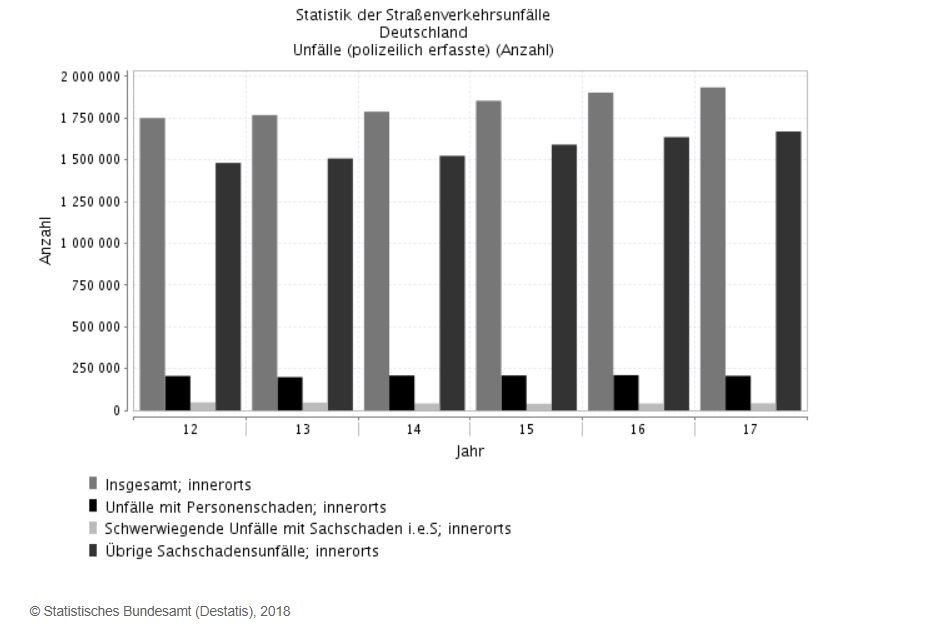
\includegraphics[width=17cm,height=13cm]{figures/Schaden}
		\caption[Anzahl der Unfälle innerorts nach Unfallkategorie]{Anzahl der innerorts Unfälle in Deutschland nach Unfallkategorie \parencite{StatistischesBundesamt.2018d}}\label{fig:Schaden}
	\end{figure}
\end{savenotes}

\subsection{Verkehrsbeteiligung an Unfällen im urbanen Raum} 
Mit ca. 59 \% sind Pkws 2016 am häufigsten an Unfällen mit Personenschaden beteiligt, am Zweithäufigsten sind Fahrräder involviert (ca. 19 \%). Die Beteiligung der Fußgänger ist mit ungefähr 8 \% relativ gering \parencite[S. 102]{StatistischesBundesamt.2018c}. Radfahrer und Fußgänger sind zwar seltener an Unfällen beteiligt, dafür kommt es aufgrund des geringen Schutzes der Beteiligten zu schwereren Folgen. Ungeschützte Verkehrsteilnehmer machen mehr als die Hälfte der Getöteten bei Unfällen, die sich innerorts ereignen, aus \parencite[S. 221]{Schreiber.2014}. Bei Unfällen mit Verletzten waren 2016 bei ca. 29 \% Radfahrer und bei ca. 12 \% Fußgänger betroffen. Den größten Anteil hatten Pkws mit ungefähr 44 \% \parencite[S. 139-142]{StatistischesBundesamt.2018c}. Hierbei muss allerdings darauf hingewiesen werden, dass es sich bei den Verletzten im Pkw größtenteils um leicht Verletzte handelt, während Unfälle mit Fahrrad- oder Fußgängerbeteiligung häufiger zu schweren Verletzungen führen \parencite[S. 145-148]{StatistischesBundesamt.2018c}. Die Verletzungsschwere ungeschützter Verkehrsteilnehmer trägt zur Annahme der \textit{Hypothese 5} in Kapitel \ref{section:Hypothesen} bei. Abbildung \ref{fig:Verkehrsbeteiligung} gibt einen Überblick über die Anzahl der Unfälle nach Art der Verkehrsbeteiligung.

\begin{savenotes}
	\begin{figure}[H]
		\centering
		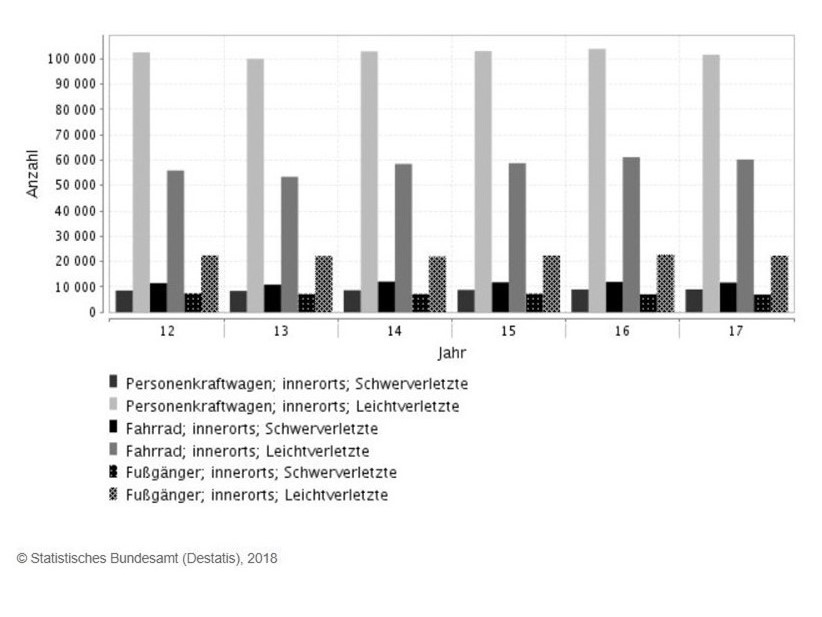
\includegraphics[width=17cm,height=13cm]{figures/Verkehrsbeteiligung}
		\caption[Anzahl der Unfälle innersorts nach Art der Verkehrsbeteiligung]{Anzahl der Verunglückten in Deutschland nach Art der Verkehrsbeteiligung und Schwere der Verletzung \parencite{StatistischesBundesamt.2018d}}\label{fig:Verkehrsbeteiligung}
	\end{figure}
\end{savenotes}

Pkw-Fahrer sind nicht nur häufig an Unfällen mit Personenschaden beteiligt, sie sind auch in mehr als der Hälfte der Fälle die Hauptverursacher. Auffällig oft sind auch Fahrradfahrer mit ca. 16 \% Hauptverursacher, während Fußgänger sehr selten die Unfallschuld tragen (4 \%) \parencite[S. 105]{StatistischesBundesamt.2018c}. In Abschnitt \ref{chapter:Unfallursachen innerorts} werden Ursachen, welche zu Unfällen führen genauer betrachtet. Hierbei liegt der Fokus auf den Fehlern der Fahrzeugführer, da sie Hauptverursacher vieler Unfälle sind. Zu den Fahrzeugführern zählen auch Fahrradfahrer, lediglich das falsche Verhalten der Fußgänger wird extra betrachtet.

\subsection{Innerorts auftretende Unfalltypen und Unfallarten }
Am häufigsten kam es 2016 bei Einbiege-/Kreuz-Unfällen, gefolgt von Unfällen im Längsverkehr zu Personenschaden. Am dritt häufigsten traten Abbiege-Unfälle auf. Diese drei Unfalltypen machten zusammen über 60 \% der Unfälle mit Personenschaden innerhalb von Ortschaften aus. Überschreitunfälle kamen seltener vor, führten dafür, da Fußgänger daran beteiligt sind, häufiger zu Getöteten oder Schwerverletzten. Da in den Statistiken nur Unfälle mit Personenschaden, Verunglückten und schwere Unfälle mit Schachschaden berücksichtigt werden machte der Typ Unfall durch ruhenden Verkehr die geringste Anzahl aus \parencite[S. 68]{StatistischesBundesamt.2017}. Hierbei muss jedoch berücksichtigt werden, dass es innerorts auch im Ruhenden Verkehr häufig zu Unfällen kommt, diese jedoch meist nur zu geringem Sachschaden führen. Diese Unfälle werden selten detailliert in den Statistiken berücksichtigt, da die Dunkelziffer nicht bei der Polizei gemeldeter Unfälle zu hoch ist. Des weiteren gibt es noch die Unfalltypen Fahrunfall und Sonstiger Unfall. Fahrunfälle machen ca. 11 \%, Sonstige Unfälle ca. 13 \% der Unfälle mit Personenschaden aus \parencite[S. 68]{StatistischesBundesamt.2017}.

Im urbanen Raum spielt die Unfallart \enquote{Zusammenstoß mit einem anderen Fahrzeug, das einbiegt oder kreuzt} die wichtigste Rolle, sie wurde 2016 bei ca. 33 \% der Unfälle mit Personenschaden angegeben. In ca. 15 \% der Fälle kam es zu einem \enquote{Zusammenstoß mit einem anderen Fahrzeug, das vorausfährt oder wartet} und zu \enquote{Unfällen anderer Art}. Unfallart von ungefähr 13 \% der Unfälle war ein \enquote{Zusammenstoß zw. Fahrzeug und Fußgänger} \parencite[S. 74]{StatistischesBundesamt.2017}.

\subsection{Charakteristiken und Besonderheiten von Unfällen im Urbanen Raum}
Fast die Hälfte der Unfälle mit Personenschaden traten 2016 an Kreuzungen (23 \%) und an Einmündungen (22 \%) auf. Die Unfälle an den Einmündungen hatten schwerere Folgen, da es etwas häufiger zu Getöteten und Schwerverletzten kam \parencite[S. 88]{StatistischesBundesamt.2017}. Dies soll bei der nachfolgenden Datenanalyse berücksichtigt werden, indem Knotenpunkte im Testgebiet genauer betrachtet werden.

Unfälle bei denen Besonderheiten der Unfallstelle erwähnt wurden traten häufig an Fußgängerfurten, Fußgängerüberwegen und Haltestellen auf. Diese drei Eigenschaften wurden 2016 bei ungefähr 7 \% der Unfälle genannt \parencite[S. 88]{StatistischesBundesamt.2017}. Bei Unfällen mit Radfahrern wird zwischen Radverkehrsanlagen auf der Fahrbahn und Radverkehrsanlagen neben der Fahrbahn unterschieden. Diese zwei Besonderheiten wurden bei ca. 5 \% der Unfälle erwähnt. Hierbei ist zu erkennen, dass sich 2016 mehr Unfälle auf Anlagen neben der Fahrbahn ereigneten \parencite[S. 88]{StatistischesBundesamt.2017}. Häufig sind Radfahrer die sich mit dem Kfz-Verkehr bewegen besser zu erkennen. Die Feststellung, dass es bei Radverkehrsanlagen neben der Fahrbahn häufiger zu Unfällen kommt führt mit zur Annahme der \textit{Hypothese 7} in Kapitel \ref{section:Hypothesen}.

\subsection{Häufige Unfallursachen innerhalb geschlossener Ortschaften}\label{chapter:Unfallursachen innerorts}
Innerorts führte das Fehlverhalten der Fahrer von Pkws mit ca. 66 \% am häufigsten zu Unfällen mit Personenschaden. Die bedeutendste Rolle spielte dabei der Fehler \enquote{Nichtbeachten der die Vorfahrt regelnden Verkehrszeichen}. Diese Unfallursache wurde 2016 allein bei 15 \% aller Unfälle innerhalb geschlossener Ortschaften genannt. Dicht dahinter folgte mit 14 \% die Ursache \enquote{Ungenügender Sicherheitsabstand}. An dritter Stelle stand die Unfallursache \enquote{Fehler beim Abbiegen} mit 13 \%. Hierbei ist auffällig, dass sich über 70 \% der Fehler beim Abbiegen nach links ereigneten. Diese Feststellung führt mit zur Annahme der \textit{Hypothese 1} in Kapitel \ref{section:Hypothesen}. Unfälle, bei denen die Unfallursache mit keiner der Zahlreichen vorgegebenen Ursachen übereinstimmen, werden der Ursache \enquote{Andere Fehler} zugeordnet. Da häufig keine genaue Ursache bestimmt werden kann machte dieser Punkt mit ca. 14 \% ebenfalls einen großen Teil der aufgenommenen Unfälle aus \parencite[S. 274-277]{StatistischesBundesamt.2018b}.

Das Fehlverhalten von Radfahrern steht an zweiter Stelle. 19 \% der Unfälle mit Personenschaden wurden 2016 durch Fehler von Radfahren verursacht. Die am häufigsten genannte Unfallursache, bei der Unfallaufnahme durch die Polizei, war \enquote{Andere Fehler der Fahrer} sie machte allein 32 \% aus. An zweiter Stelle wurde die Ursache \enquote{Falsche Straßenbenutzung} mit 23 \% am häufigsten genannt. Oft erwähnt wurde, mit ca. 14 \%, auch der Fehler \enquote{Verbotswidrige Benutzung der Fahrbahn oder anderer Straßenteile} \parencite[S. 274-277]{StatistischesBundesamt.2018b}. Es ist zu erkennen, dass bei den Radfahren im Vergleich zu den Pkw-Fahrern andere Unfallursachen häufig auftreten. Es kommt oft zu Unfällen mit Radfahrern, wenn diese übersehen werden, weil sie z.B. verbotswidrig den Radweg in die falsche Richtung befahren oder den Fußweg benutzen. Die falsche Benutzung von Straßen ist mit einem Pkw deutlich schwieriger und kommt deshalb als Unfallursache nur selten vor.

Fußgänger sind zwar seltener an Unfällen beteiligt, sollen aber aufgrund der häufig schwereren Unfallfolgen nicht vernachlässigt werden. Die am häufigsten genannte Unfallursache bei fehlerhaftem Verhalten der Fußgänger ist \enquote{Falsches Verhalten beim Überschreiten der Fahrbahn}. Allein diese Ursache wurde 2016 bei fast 80 \% der Unfälle erwähnt. Um einen besseren Überblick über das Unfallgeschehen zu bekommen wurde die Ursache durch genauere Beschreibungen, wie die Fahrbahn überquert wird, ergänzt. Am mit Abstand meisten Unfälle ereigneten sich, wenn Fußgänger die Fahrbahn überquerten ohne dabei auf den Fahrzeugverkehr zu achten. Unfall anfällig war auch das plötzliche hervortreten hinter Sichthindernissen. Häufig kam es auch zu falschem Verhalten an Stellen, an denen der Fußgängerverkehr durch Polizeibeamte oder Lichtzeichen geregelt war \parencite[S. 304]{StatistischesBundesamt.2018b}. Hierbei war vor allem das überqueren einer Fußgängerampel bei rot von Bedeutung \parencite[S. 222]{Schreiber.2014}. Diese Zahlen tragen mit zur Annahme der \textit{Hypothese 8} in Kapitel \ref{section:Hypothesen} bei. Weitere 12 \% der Unfallursachen wurden ähnlich wie bei den Pkw- und Radfahrern durch \enquote{Andere Fehler} angegeben \parencite[S. 304]{StatistischesBundesamt.2018b}.

Unfälle können jedoch nicht nur von Fahrzeugführern oder Fußgängern verursacht werden sondern auch durch allgemeine Ursachen. Hierzu zählen Straßenverhältnisse, Witterungseinflüsse, Hindernisse und sonstige Unfallursachen. Die meisten Unfallursachen wurden 2016 in der Kategorie Hindernisse und sonstige Unfallursachen genannt, wobei die zweite Ursache wesentlich häufiger vorkommt. An zweiter Stelle stehen die Straßenverhältnisse, hier wird am Häufigsten Regen als Unfallursache angegeben gefolgt von Schnee und Eis. Bei den Witterungseinflüssen machte die Unfallursache \enquote{blendende Sonne} mit Abstand den größten Teil aus (83 \%). Starker Regen, Hagel, Schneegestöber, etc. werden bei den Witterungseinflüssen an Zweiterstelle genannt, sie machten mit 10 \% jedoch einen wesentlich geringeren Teil der Unfallursachen, die zu Personenschaden führen, aus \parencite[S. 305]{StatistischesBundesamt.2018b}. Der hohe Einfluss durch \enquote{blendende Sonne} stellt auch \Textcite[S. 151]{Grundl.2005} in seiner Arbeit fest und führt zur Annahme der \textit{Hypothese 9} in \ref{section:Hypothesen}.

Bei den genannten Zahlen muss berücksichtigt werden, dass statistische Informationen allein nicht gut genug sind um relevante oder kritische Fahrsituationen festzustellen. Sie stellen nur das Ergebnis eines Unfalls dar, es wird jedoch nicht untersucht, wie es zu dem Unfall kam. Zudem liegt der Fokus auf Unfällen mit Personenschaden. Für die folgende Datenanalyse werden deshalb die durch die polizeiliche Unfallaufnahme vorliegenden Informationen genauer betrachtet. 

\section{Urbane Fahrsituationen und ihre Sicherheitsbewertung}\label{section:urbane Fahrsituationen und ihre Sicherheitsbewertung}
In Kapitel \ref{chapter:Verkehrsunfälle in Deutschland} wurden bereits Unfälle und Unfallzahlen innerhalb geschlossener Ortschaften vorgestellt. Es wurde jedoch nicht genauer darauf eingegangen, an welchen Stellen im Straßennetz und in was für Konstellationen sich häufig Unfälle ereignen. \enquote{Die Charakteristik des Unfallgeschehens ist auf Abschnitten der freien Strecke und Knotenpunkten grundsätzlich unterschiedlich} \parencite[S. 83]{Aurich.2015}. Deshalb werden in diesem Kapitel urbane Fahrsituationen und mögliche Konfliktpunkte, vor allem an Kreuzungen, noch detaillierter betrachtet.

\subsection{Konfliktpunkte an Knotenpunkten}\label{subsection:Konfliktpunkte an Knotenpunkten}
Da sich 36 \% der urbanen Fahrsituationen an Knotenpunkten ereignen \parencite[S. 40]{Gerstenberger.17.02.2015} treten in diesem Bereich häufig Konflikte auf. Hierbei enthalten vor allem die Fahrsituationen Kreuzen, Einbiegen und Abbiegen ein hohes Konfliktpotential, da sich vielfältige Überschneidungen der möglichen Bewegungsbahnen ergeben können \parencite[S. 83]{Reichart.2001}. Bei dem Fahrmanöver Abbiegen nach links kommt es am häufigsten zu möglichen Konfliktpunkten, nur geringfügig weniger Konflikte treten beim Geradeausfahren bzw. Kreuzen auf. Am wenigsten Konflikte ereignen sich beim Rechtsabbiegen. In Abbildung \ref{fig:Konfliktpunke am Knotenpunkt} werden mögliche Konfliktpunkte und die entsprechenden Verkehrsbeteiligten dargestellt. Sobald bei einem Fahrmanöver andere Verkehrsteilnehmer berücksichtigt werden müssen steigt die Beanspruchung des Fahrers \parencite[S. 9]{Mages.2008}. \Textcite[S. 84]{Reichart.2001} bezeichnet das Linksabbiegen bzw. - einbiegen als eine der Fahraufgaben, die am schwierigsten und unfallträchtigsten ist.

\begin{savenotes}
	\begin{figure}[H]
		\centering
		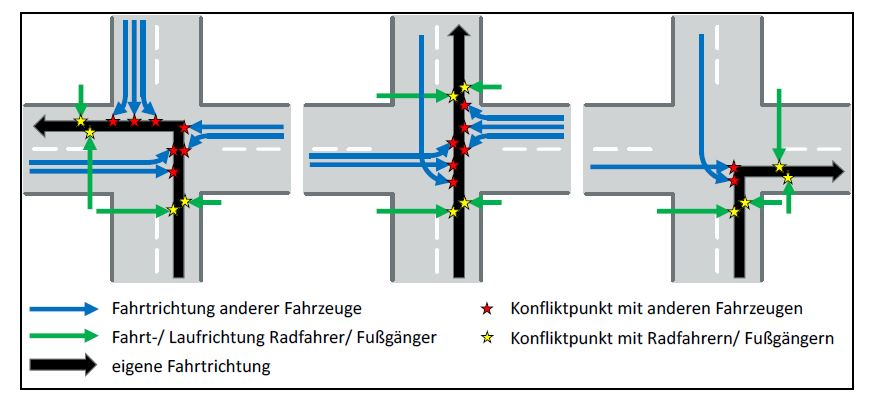
\includegraphics[width=15cm,height=7cm]{figures/Konfliktpunkte}
		\caption[Mögliche Konfliktpunkte am Knotenpunkt beim Linksabbiegen, Geradausfahren und Rechtsabbiegen]{Mögliche Konfliktpunkte am Knotenpunkt beim Linksabbiegen, Geradausfahren und Rechtsabbiegen \parencite[S. 41]{Gerstenberger.17.02.2015}}\label{fig:Konfliktpunke am Knotenpunkt}
	\end{figure}
\end{savenotes}

Bei den Konfliktpunkten in Abbildung \ref{fig:Konfliktpunke am Knotenpunkt} treten beim Linksabbiegen am Häufigsten Unfälle mit entgegenkommenden Fahrzeugen auf, beim Geradeausfahren dagegen mit Verkehrsteilnehmern von rechts. Das Fahrmanöver Rechtsabbiegen führt am Häufigsten zu Unfällen mit von rechts kommenden Radfahrern und Fußgängern. Nicht berücksichtigt wurden mögliche Konflikte mit dem Nachfolgenden Verkehr oder mit Fahrzeugen auf benachbarten Fahrstreifen.

Insgesamt ereignen sich 75 \% aller Unfälle an Knotenpunkten beim Abbiegen und das obwohl bei einer Fahrt durchschnittlich nur an jedem fünften Knotenpunkt nach rechts oder links abgebogen wird \parencite[S. 101-102]{Gerstenberger.17.02.2015}. Beim Linksabbiegen kommt es dabei, auf Grund der höheren Komplexität des Abbiegevorgangs, häufiger zu Unfällen als beim Rechtsabbiegen \parencite[S. 117]{Grundl.2005}. \Textcite[S. 15]{Mages.2008} stellt bei seinen Analysen fest, dass ungefähr 93 \% der Unfälle die beim Einbiegen/Kreuzen entstehen auf die Unfalltypen 301, 302, 303, 321 und 322 in Abbildung \ref{fig:Einbiege-Unfall} entfallen. Während an Kreuzungen die meisten Unfälle durch Linksabbieger verursacht werden, kommt es an Einmündungen häufiger zu Unfällen durch Rechtsabbieger \parencite[S. 102-103] {Gerstenberger.17.02.2015}.

Einen wesentlichen Einfluss auf den wahrgenommenen Schwierigkeitsgrad stellt neben der Komplexität eine vorhandene Sichtbehinderung dar. Häufig ist es dem Fahrer aufgrund von ständigen, z.B. Häusern, oder beweglichen, z.B. parkende Fahrzeuge, Sichthindernissen nicht möglich sich einen ausreichenden Überblick über die Kreuzung zu verschaffen. Dies führt dazu, dass Verkehrsteilnehmer die vorfahrtsberechtigt sind erst zu spät oder gar nicht erkannt werden \parencite[S. 9]{Mages.2008}. Besonders häufig kommt es hierbei zu schweren Unfällen mit Fußgängern und Fahrradfahrern. Unfälle beim Linksabbiegen können auch zu schweren Folgen führen. Hierbei spielen Sichtbehinderungen jedoch nicht die entscheidende Rolle. Die schweren Folgen sind auf  hohe Geschwindigkeiten der entgegenkommenden Verkehrsteilnehmer zurückzuführen \parencite[S. 417]{AbdelAty.2005}. Ein Ansatz um Fahrsituationen an Knotenpunkten besser beurteilen zu können ist es, sie in unterschiedliche Segmente einzuteilen. \Textcite[S. 112]{Gerstenberger.17.02.2015} unterscheidet zwischen den Segmenten: Annähern, Verzögern, Querung I, Querung II und Verlassen. Die Segmente werden hierbei in der genannten Reihenfolge durchfahren. Jede Teilaufgabe innerhalb eines Segments führt zu einer bewussten Entscheidung, hierbei können mögliche Fehlerquellen entstehen \parencite[S. 25]{Gerstenberger.17.02.2015}. %Gestenberger eräutert die einzelnen Segmente noch genauer. Evtl. noch detaillierter Beschreiben, falls dies zum besseren Verständnis beiträgt.

Untersuchungen von \Textcite[S. 112]{Gerstenberger.17.02.2015} haben ergeben, dass die häufigste Unfallursache beim Unfallverursacher das Missachten der Vorfahrtsregelung ist, gefolgt von Fehlern beim Abbiegen. Die Unfallursachen welche beim Unfallgegner am meisten genannt werden sind falsche Straßenbenutzung, Geschwindigkeitsmissachtung und Missachtung der Vorfahrtsregelung. 

Innerorts werden in einer Stunde Fahrt ca. 80 bis 120 Knotenpunkte passiert, davon wird ca. die Hälfte mit einer Lichtsignalanlage geregelt \parencite[S. 114]{Reichart.2001}. Durch den Einsatz von Lichtsignalanlagen können die Konfliktpunkte an plangleichen Knotenpunkten reduziert werden \parencite[S. 83]{Reichart.2001}. Dies geschieht, indem gewisse Verkehrsströme nie gleichzeitig grün erhalten dürfen. \Textcite[S. 417]{AbdelAty.2005} stellt bei seinen Untersuchungen hingegen fest, dass sich an Kreuzungen mit LSA häufiger Unfälle ereignen als an Kreuzungen mit Stoppschild oder Vorfahrtachtenzeichen. Dies kann daran liegen, dass lichtsignalgeregelte Knotenpunkte meist ein wesentlich höheres Verkehrsaufkommen aufweisen. Im Folgenden Kapitel werden Konfliktpunkte an Knotenpunkten mit einer LAS genauer betrachtet.


\subsubsection{Konflikte im Bereich von lichtsignalisierten Knotenpunkten}\label{chapter:Knotenpunkte mit LSA}

Im Bereich von lichtsignalisierten Knotenpunkten stellen Abbiegeunfälle den häufigsten Unfalltyp dar. Sowohl beim Links- als auch beim Rechtsabbiegen treten häufig Konfliktpunkte auf. Beim Linksabbiegen kommt es vor allem zu Konflikten mit dem gleichzeitig freigegebenen Gegenverkehr \parencite[S. 273]{Schreiber.2016}, Unfalltyp 21 in Abbildung \ref{fig:Abbiege-Unfall}. Es treten aber auch Konflikte mit dem Fußgänger- und Radverkehr auf parallel freigegebenen Nebenanlagen auf. Diese werden in den Unfalltypen 221 bis 224 in Abbildung \ref{fig:Abbiege-Unfall} dargestellt. Beim Rechtsabbiegen kommt es ebenfalls oft zu Konflikten mit Radfahrern und Fußgängern, die sich parallel bewegen \parencite[S. 273]{Schreiber.2016}. Sie Stellen die Unfalltypen 241 bis 244 in Abbildung \ref{fig:Abbiege-Unfall} dar. Zudem spielen Unfälle mit dem nachfolgenden Verkehr eine große Rolle. Hierbei handelt es sich meist um Auffahrunfälle, wegen zu geringem Sicherheitsabstand.

\begin{savenotes}
	\begin{figure}[H]
		\centering
		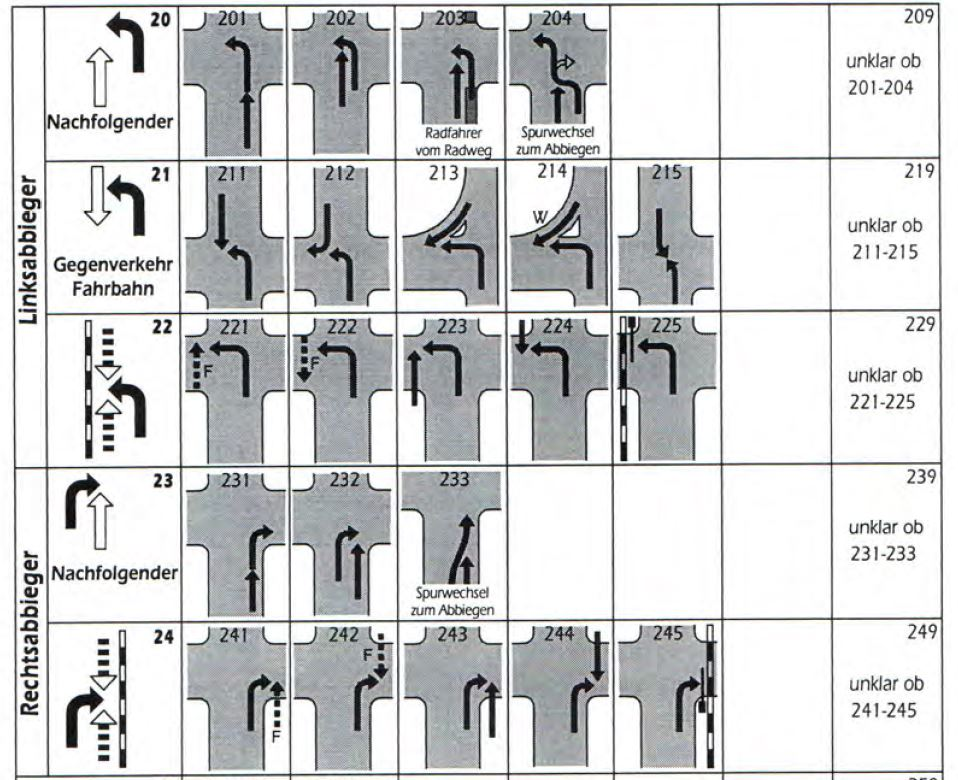
\includegraphics[width=13cm,height=11cm]{figures/Abbiege-Unfall}
		\caption[Unfalltyp 2 Abbiege-Unfall]{Mögliche Unfalltypen beim Abbiegen \parencite[S. 11]{GesamtverbandderDeutschenVersicherungswirtschafte.V..2016}. }\label{fig:Abbiege-Unfall}
	\end{figure}
\end{savenotes}

Am zweithäufigsten kommt es an Knotenpunkten mit LAS zu Unfällen im Längsverkehr. Bei fast 70 \% der Unfälle wird hier die Unfallursache \enquote{ungenügender Sicherheitsabstand} angegeben, es kommt daher häufig zu Auffahrunfällen mit dem Vorausfahrenden oder einem Fahrzeug, das bereits an einer Ampel wartet. Darauf folgen die Ursachen \enquote{Fehler beim Fahrstreifenwechsel} und \enquote{unangepasste Geschwindigkeit} \parencite[S. 273]{Schreiber.2016}. Bei Unfällen im Längsverkehr hat die Verkehrsstärke einen zusätzlichen Einfluss auf die Zahl der Unfälle. Hier sind vor allem leichtere Unfälle betroffen \parencite[S. 86]{Aurich.2015}. Diese Informationen führen zur Annahme der \textit{Hypothese 3} in Kapitel \ref{section:Hypothesen}.

Einbiegen-/Kreuzen-Unfälle sollten an Knotenpunkten mit einer Lichtsignalanlage eigentlich nicht auftreten. Kreuzende Verkehrsströme, sogenannte nicht verträgliche Ströme, dürfen nicht in der gleichen Signalphase grün erhalten. Trotzdem ereignen sich auch solche Unfälle. Diese werden dann durch die Unfallursache Rotlichtverstoß verursacht \parencite[S. 274]{Schreiber.2016}. 

Die oben genannten Konfliktpunkte können zum Teil durch einfache Maßnahmen verringert werden. An stark frequentierten Knotenpunkten sollte innerorts immer gesichertes Linksabbiegen zur Anwendung kommen \parencite[S. 275]{Schreiber.2016}. Werden die Linksabbieger an Lichtsignalanlagen mit eigenem Signal in einer separierten Phase geführt ist es möglich die oben genannten Konfliktpunkte zu reduzieren. Linksabbiegestreifen ohne eine eigene Signalphase tragen nicht zur Reduktion der Konfliktpunkte bei. Dies führt zur Annahme der \textit{Hypothese 2} in Kapitel \ref{section:Hypothesen}. Konflikte mit Radfahrern und Fußgängern können verringert werden, indem der Sichtkontakt zum Kraftfahrzeug gewährleistet wird. Ist dies nicht möglich können auch hier gesonderte Signalisierungen der Abbieger und Radfahrer/Fußgänger zum Einsatz kommen. Werden Radfahrer auf Radverkehrsanlagen in Nähe der Fahrbahn geführt kann der Sichtkontakt ebenfalls verbessert werden. Sobald Radwege eine Furtabsetzung, die größer als zwei Meter ist, haben kommt es zu Beeinträchtigungen der Sichtbeziehungen \parencite[S. 276f]{Schreiber.2016}.

\subsubsection{Konflikte an Knotenpunkten ohne Lichtsignalanlage}\label{chapter:Knotenpunkte ohne LSA}
An innerstädtischen Knotenpunkten ohne \ac{LSA} kommt es am häufigsten bei Einmündungen und Kreuzungen mit der Regel Vorfahrt gewähren zu Unfälle. Hierbei kann das Einbiegen aus einer wartepflichtigen Straße ohne \ac{LSA} als eine der schwierigsten Fahraufgaben eingestuft werden \parencite[S. 90]{Reichart.2001}. Am meisten Kollisionen ereignen sich, wenn es zu einem Konflikt mit dem vorfahrtsberechtigten Querverkehr kommt. Der Unfalltyp 342, Konflikt mit einem querenden Radfahrer von Rechts, welcher in Abbildung \ref{fig:Einbiege-Unfall_Rad} dargestellt wird tritt dabei am häufigsten auf. An zweiter und dritter Stelle steht der Konflikt mit einem bevorrechtigten Fahrzeug von links. Hier spielen die Unfalltypen 302 und 301 die wichtigste Rolle, sie werden in Abbildung \ref{fig:Einbiege-Unfall} dargestellt. Etwas seltener kommt es zu Konflikten mit querenden Fahrzeugen von rechts. Konfliktpunkte ereignen sich jedoch nicht nur mit dem Querverkehr sondern auch mit nachfolgenden Fahrzeugen beim Linksabbiegen, Unfalltyp 201 und 202 in Abbildung \ref{fig:Abbiege-Unfall}.

\begin{savenotes}
	\begin{figure}[H]
		\centering
		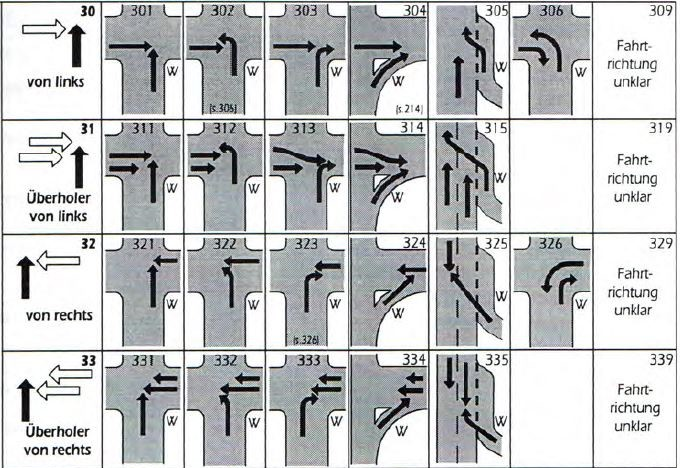
\includegraphics[width=13cm,height=9cm]{figures/Einbiege-Unfall}
		\caption[Unfalltyp 3 Einbiegen/Kreuzen-Unfall]{Mögliche Unfalltypen beim Einbiegen/Kreuzen \parencite[S. 13]{GesamtverbandderDeutschenVersicherungswirtschafte.V..2016}}\label{fig:Einbiege-Unfall}
	\end{figure}
\end{savenotes}

\subsection{Urbane Fahrsituationen mit geringen Geschwindigkeiten}\label{Urabane Fahrsituationen mit geringen Geschwindigkeiten}
Innerorts kommt es häufig zu kleineren Unfällen mit geringen Geschwindigkeiten. Wie bereits erwähnt ist die Dunkelziffer der nicht Erfassten Unfälle mit Sachschaden sehr hoch. Viele Unfälle werden gar nicht erst gemeldet und diejenigen die von der Polizei aufgenommen werden beinhalten meist zu wenig Information über den Unfallablauf. Ein Grund für die oftmals nicht vorhanden Informationen ist, dass die vorhandenen Unfalltypen für Unfälle mit Personenschaden ausgelegt sind. \Textcite[S. 58]{Gschwendtner.2015} hat sich detaillierter mit Fahrsituationen und Konflikten befasst die zu Unfällen mit Sachschaden führen und eine neue Unfalltypen Kategorie \enquote{Detaillierung Sachschaden} aufgestellt. Diese wird in vier weitere Untergruppen (Rangieren, Konflikte mit Objekten, Konflikte beim Ein- und Ausparken und weitere Konflikte) aufgeteilt. Somit wird es ermöglicht Situationen mit niedrigen Geschwindigkeiten genauer zu klassifizieren.

Besonders häufig ereignen sich Unfälle beim Rückwärtsfahren. Hier bei kommt es ähnlich oft zum Konflikt mit einem kleinen Objekt, bis zu 10 cm Durchmesser, wie zum Konflikt mit einem großen Objekt, z.B. einer Wand oder Mauer. Häufig ereignen sich auch Konflikte mit einem mittleren Objekt. Hier führt die Konstellation Objekt auf der rechten Seite des Fahrzeugs und Lenkeinschlag nach rechts häufig zu Konflikten. Seltener kommt es beim Vorwärtseinparken zu einem Konflikt mit der Bordsteinkante oder zu Konfliktpunkten beim Rückwärtsausparken aus einer Quer- bzw. Schrägparklücke. Die Unfalltypen sind so gestaltet, dass nicht nur die Fahrtrichtung und der Lenkeinschlag angegeben wird, sondern auch die Objektgröße und die Position des Objekts bzw. des Fahrzeugs mit dem es zu einem Konflikt kam \parencite[S. 58-61]{Gschwendtner.2015} Die vier oben genannten Konfliktsituationen stellen nur einen kleinen Auszug dar. Betrachtet man den bereits definierten Typ Unfall durch ruhenden Verkehr sind zwei Unfallkonstellationen auffällig. Hierbei kommt es häufig zu Konflikten von sich im fließenden Verkehr bewegenden Fahrzeugen, mit  Fahrzeugen die längs am Straßenrand parken oder Ausparken \parencite[S. 53]{Vollrath.2006}. Hieraus ergibt sich \textit{Hypothese 4} in Kapitel \ref{section:Hypothesen}.

\subsection{Konfliktpunkte zwischen Kraftfahrzeugen und Radfahrern}
In Kapitel \ref{subsection:Konfliktpunkte an Knotenpunkten} wurden bereits Konfliktpunkte mit Radfahrern erwähnt. Da innerorts, trotz geringerer Verkehrsbeteiligung, jeder vierte Verunglückte ein Radfahrer ist \parencite[S. 303]{Schreiber.2014b} und die Anzahl an Verunglückten bei Radfahrern in den letzten Jahren weniger stark abgenommen hat \parencite[S. 7]{Below.2016} werden Unfälle mit der Beteiligung von Fahrradfahrern hier nochmals genauer betrachtet. Zu Beginn soll drauf hingewiesen werden, dass Radfahrunfällen, besonders bei Alleinunfällen und Unfällen mit geringen Verletzungen häufig nicht bei der Polizei gemeldet werden. Laut einer Studie von \Textcite[S. 80]{Below.2016} sind möglicherweise bis zu 88 \% der Fahrradunfälle, die zu einer Verletzung des Radfahrers führen, nicht in den Statistiken enthalten. Es besteht also eine erhebliche Dunkelziffer in diesem Bereich. Im Folgenden werden Knotenpunkte mit und ohne Lichtsignalanlage gemeinsam bei der Analyse von Konfliktpunkten mit Radfahrern berücksichtigt.

Ungefähr 90 \% \parencite[S. 10]{Below.2016} der Radfahrer verunglücken innerhalb von Ortschaften dabei sind sie laut \Textcite[S. 303]{Schreiber.2014b} beim Einbiegen-/Kreuzen am Häufigsten an Unfällen beteiligt. Der bei den lichtsignalisierten Knotenpunkt mit Abstand am Häufigsten auftretende Abbiegeunfall steht hier nur an zweiter Position. Unfälle beim Einbiegen/Kreuzen entstehen, wenn es zu einem \enquote{Konflikt zwischen einem einbiegenden oder kreuzenden Wartepflichtigen und einem Vorfahrtsberechtigten} \parencite[S. 12]{GesamtverbandderDeutschenVersicherungswirtschafte.V..2016} kommt. Da sowohl \ac{Kfz}- als auf Radfahrer häufig ihrer Wartepflicht nicht nachkommen sind Konfliktpunkte vor allem an Knotenpunkten mit der Reglung rechts-vor-links oder Vorfahrtachten unumgänglich. Ein Beispiel für häufige Konfliktpunkte mit Radfahren sind die Unfalltypen 341 bis 344 die in Abbildung \ref{fig:Einbiege-Unfall_Rad} dargestellt werden.

\begin{savenotes}
	\begin{figure}[H]
		\centering
		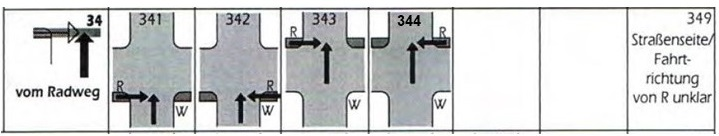
\includegraphics[width=13cm,height=2cm]{figures/Einbiege-Unfall_Rad}
		\caption[Unfalltyp 3 Einbiegen/Kreuzen-Unfall mit Radfarerbeteiligung]{Mögliche Unfalltypen, beim Einbiegen/Kreuzen mit der Beteiligung von Radfahrern \parencite[S. 13]{GesamtverbandderDeutschenVersicherungswirtschafte.V..2016}}\label{fig:Einbiege-Unfall_Rad}
	\end{figure}
\end{savenotes}

Beim Abbiegen muss \enquote{ein abbiegendes Fahrzeug dem geradeaus fahrenden Radfahrer die Vorfahrt gewähren} \parencite[S. 303]{Schreiber.2014b}. Hierbei kommt es vor allem beim Rechtsabbiegen häufig vor, dass Radfahrern die Vorfahrt genommen wird. Teilweise kommt es aufgrund von Sichthindernissen trotz vorsichtigem Verhalten der Kraftfahrzeugführer zu Unfällen. Hierbei sind vor allem Situationen, in denen sich Radfahrer mit hoher Geschwindigkeit von Hinten nähern besonders kritisch. Hinzu kommt, dass Radfahrer häufig den Radweg in die Falsche Richtung befahren oder den Knotenpunkt nicht innerhalb der vorgeschriebenen Markierung überqueren. Mit diesen Situationen rechnet der Fahrer eines Kraftfahrzeugs nicht zwangsläufig und es kann passieren, dass er den Radfahrer zu spät erkennt. Häufig kommt es auch zu Konfliktsituationen, wenn Kfz-Fahrer den Schulterblick beim Abbiegen nicht durchführen und aufgrund dessen Radfahrer übersehen. Beim Linksabbiegen kommt es deutlich seltener zu Unfällen mit Radfahrern, da die Bereiche häufig für den Kfz-Fahrer besser einsehbar sind. Dies führt mit zur Annahme der \textit{Hypothese 6} in Kapitel \ref{section:Hypothesen}.

Möglichkeiten diese Konflikte zu reduzieren zeichnen sich auch hier durch die Vermeidung von Sichthindernissen und einer Führung der Radfahrer auf der Fahrbahn im Mischverkehr oder zumindest in Fahrbahnnähe aus. Zusätzlich müssen Sichtfelder für den Schulterblick freigehalten werden und eine entsprechende Gestaltung der Radwege im Kreuzungsbereich (z.B. Roteinfärbung) kann zu erhöhter Aufmerksamkeit führen \parencite[S. 309]{Schreiber.2014b}. Radfahrer sind in 41,5 \% \parencite[S. 10]{Below.2016} der Fälle selbst Hauptverursacher, es besteht also auch auf Seiten der Radfahrer ein großes Unfallvermeidungspotential, wenn sie ihr Verhalten anpassen und sich regelkonform verhalten. Das am Häufigsten auftretende Fehlverhalten auf Seiten der Radfahrer stellt die Falsche Straßenbenutzung dar.

\subsection{Konflikte außerhalb von Knotenpunkten}
Außerhalb von Knotenpunkten treten vor allem die Unfalltypen Fahrunfall und Unfall im Längsverkehr auf. Innerhalb geschlossener Ortschaften spielt der Typ Fahrunfall eine geringe Rolle und soll hier nicht weiter beachtet werden. Bei Unfällen im Längsverkehr kommt es, aufgrund des dichten Stadtverkehrs, häufig zu Unfälle die durch Abstandsfehler oder Fehler beim Spurwechsel auf mehrstreifigen Fahrbahnen entstehen \parencite[S. 25]{Schmidt.2010}.

Überschreiten-Unfälle stellen einen weiteren Unfalltyp dar, der sich auch außerhalb von Knotenpunkten ereignet. Sie treten oft an Punkten von großem Interesse auf, an denen Fußgänger die Fahrbahn queren ohne Querungshilfen zu verwenden. Hierbei kann es sich um Unfälle in einer Einkaufsstraße mit vielen Geschäften auf beiden Fahrbahnseiten, oder Bereiche in der Nähe von Haltestellen des \ac{ÖPNV} handeln. Dies trägt mit zu Annahme der \textit{Hypothese 8} in Kapitel \ref{section:Hypothesen} bei. Bereiche an denen linienfaht querende Fußgänger verunglücken können auch als \enquote{Unfallhäufungslinien} bezeichnet werden \parencite[S. 18]{ForschungsgesellschaftfurStraenundVerkehrswesen.2012}. Im Vergleich zu Unfällen an Knotenpunkten treten Überschreiten-Unfälle jedoch eher selten auf.

\subsection{Konfliktpunkte bei Nacht}
Da das menschliche Sehvermögen nachts eingeschränkt ist, treten in der Nacht höhere Unfallraten auf als am Tag. Viele dieser Nachtunfälle ereignen sich außerorts. Lediglich Unfällen mit Fußgängerbeteiligung treten nachts in 90 \% der Fällen innerorts auf. Im Winter ereignen sich aufgrund der länger anhaltenden Dunkelheit mehr Unfälle bei Nacht. Zudem treten in den Nächten von Freitag und Samstag bzw. Samstag auf Sonntag mehr Unfälle auf  \parencite[S. 12]{DEKRA.2017}. Sowohl bei Tag als auch bei Nacht ist die mittlere Unfallschwere bei Unfällen die sich innerhalb geschlossener Ortschaften ereignen am geringsten \parencite[S. 18]{DEKRA.2017}. Neben Überschreitunfällen ereignen sich Nachts innerorts Unfälle beim Einbiegen-Kreuzen und im Längsverkehr \parencite[S. 26]{DEKRA.2017}.


\section{Menschliches Verhalten im Straßenverkehr}
Wie bereits erwähnt wird die Mehrheit der Unfälle durch menschliche Fehler ausgelöst. Um zu verstehen, wie es zu Fehlern im Straßenverkehr kommt, müssen zunächst die Aufgaben betrachtet werden, die ein Fahrer bei der Fahrzeugführung erfüllen muss. Zusätzlich ist zu beachten, dass verschiedene Situationen, je nach Komplexität, zu einer unterschiedlich starken Belastung der Fahrer führen. Diese beiden Punkte sollen in Kapitel \ref{Der Mensch als Fahrzzeugführer} betrachtet werden. Kapitel \ref{Fehler des Menschen bei der Verkehrsbeteiligung} befasst sich mit der Entstehung der Fehler und gibt einen Ausblick, was bei der Unfallaufnahme im Bezug auf menschliche Fehler berücksichtigt werden muss.

\subsection{Der Mensch als Fahrzeugführer}\label{Der Mensch als Fahrzzeugführer}
Die Fahranforderungen an den Menschen können durch das Drei-Ebenen-Modell der Fahrzeugführung beschrieben werden. Die drei Komponenten Navigation, Führung und Stabilisierung bilden das Modell und stellen unterschiedliche Anforderungen an den Fahrer. Die Aufgaben der drei Ebenen können nicht unabhängig voneinander betrachtet werden, da sie sich gegenseitig beeinflussen bzw. aufeinander aufbauen. Die Navigationsebene beinhaltet z.B. die Wahl der Fahrtroute um ein bestimmtes Ziel zu erreichen. Die Führungsebene umfasst dagegen für die Umsetzung der ausgewählten Route notwendigen Aufgaben (z.B. Abbiegen an einem Knotenpunkt) und auf der Stabilisierungsebene werden die Fahranforderungen für die Längs- und Querführung des Fahrzeugs zusammengefasst (z.B. Lenk- und Bremsvorgänge) \parencite[S. 16]{Gerstenberger.17.02.2015}. Zusätzlich kann noch nach dem Grad der kognitiven Beanspruchung unterschieden werden. Die Verhaltensweisen treten entweder wissensbasiert, regelbasiert oder fähingkeitsbasiert auf. Tätigkeiten auf der Navigationsebene sind eher wissensbasiert, fähigkeitsbasierte Tätigkeiten sind auf der Stabilisierungsebene zu erkennen und regelbasierte auf der Führungsebene \parencite[S. 45]{Grundl.2005}.

Der Bremsvorgang stellte ein wichtiges Element der Führungsebene dar. Nur wenn der Fahrer \enquote{rechtzeitig} bremst können Unfälle verhindert oder ihre Folgen verringert werden. Der Bremsvorgang wird in drei Reaktionsphasen eingeteilt: Reaktionsgrundzeit (ca. 0,45 s), Umsetzzeit (ca. 0,19 s) und Ansprechzeit (ca. 0,005 s). Die genannten Werte stellen Mittelwerte dar. Die gesamte Dauer eines Bremsvorgangs liegt ungefähr zwischen 0,40 s und 0,85 s. Bevor der Bremsvorgang eingeleitet werden kann vergeht noch die Zeit zwischen der peripheren Wahrnehmung und der Objektfixierung. Hierfür werden im Schnitt 0,48 s benötigt. Zusammenfassend kann gesagt werden, dass mit der Gefahrenerkennung die Reaktionsdauer beginnt \parencite[S.153]{Burg.2017}. Rund die Hälfte aller Kollisionen könnte eben noch verhindert werden, wenn jeder Beteiligte sein unfallvermeidendes Fahrmanöver 0,5-1,0 s früher einleiten würde. Hieraus ist zu erkennen, dass bereits winzige Zeitspannen eine erhebliche Wirkung auf die Verkehrssicherheit haben \parencite[S. 271]{Burg.2017}.

Häufig wird der Mensch als schwächstes Glied im Bereich des Verkehrssystems angesehen, da er Verursacher von rund 95 \% der Kollisionen ist. Diese Auffassung sollte jedoch relativiert werden, da ein Aufprall kaum monokausal erklärt werden kann. Betrachtet man das Verkehrsgeschehen als Gesamtsituation und bezieht das Fahrzeug und die Umwelt mit ein kann der Fahrzeugführer ohne Rücksicht auf die Gesamtsituation und ihre Entstehungsbedingungen selten als alleiniger Unfallverursacher genannt werden \parencite[S. 269]{Burg.2017}. Die Handlungszuverlässigkeit des Menschen nimmt jedoch ab, wenn die Belastung durch die Fahraufgabe und Begleitumstände die aktuelle Leistungsmöglichkeit übersteigen. Die Belastung mit der der Straßenverkehr auf den Fahrer einwirkt kann durch statische oder dynamische Faktoren hervorgerufen werden. Im urbanen Raum zählen die Art der Vorfahrtssituation und Signalisierung ebenso wie die Art der Bebauung und z.B. der Straßenbelag zu den statischen Faktoren. Dynamische Einwirkungen haben z.B die Verkehrsstärke, das Fahrmanöver, Wetterbedingungen und Nebenaufgaben. Hierbei ist zu beachten, dass die Schwierigkeit der Fahraufgaben und somit die Belastung auf den Fahrer mit verschlechterten Sichtbedingungen, abnehmendem Kraftschluss zwischen Reifen und Fahrbahn, geringer Vorhersehbarkeit von Störgrößen, zunehmender Informationskomplexität und zunehmender Entscheidungskomplexität erhöht wird \parencite[S. 132]{Reichart.2001}. Hierbei darf nicht vernachlässigt werden, dass auch zu geringe Belastungen nicht optimal sind. Sie können zur Monotonie führen. Der Bereich der optimalen Handlungszuverlässigkeit tritt deshalb bei einer mittleren Belastung auf \parencite[S. 270]{Burg.2017}. Im Folgenden sollen Fehler des Menschen die zur Entstehung eines Unfalls beitragen können betrachtet werden.

\subsection{Fehler des Menschen bei der Verkehrsbeteiligung}\label{Fehler des Menschen bei der Verkehrsbeteiligung}
Bei der Teilnahme am Straßenverkehr kommt es immer wieder zu Fehlern durch Unachtsamkeit oder häufig auch durch Überforderung. Handlungen die nicht an vorliegende Situationen angepasst sind und zu Schäden führen werden als Fehler bezeichnet \parencite[S. 17]{Gerstenberger.17.02.2015}. Es existieren unabhängig vom durchgeführten Fahrmanöver sechs Arten von Fehlhandlungen und Ursachen. Es kann sich dabei um die Vernachlässigung oder Nicht-Ausführung bestimmter Fahraufgaben, Fehlanpassung der Manöver an die Fahrsituation, Fehlinterpretation der Fahrsituation, Fehleinschätzung des Verhaltens anderer Verkehrsteilnehmer,  das bewusstes Eingehen von Risiken und Verstößen oder die fehlerhafte Ausführung von Handlungen eignen \parencite[S. 32f]{Vollrath.2006}. %Auf S.33 ist auch noch eine Tabelle dargestellt, in welcher die Fehlhandlungen Aufgaben beim Fahren und Situation zugeordnet werden.

Während der erfolgreichen und sicheren Bewältigung einer Fahraufgabe müssen viele Details berücksichtigt werden. Das führt häufig zu einer geteilten Aufmerksamkeit, da die Aufmerksamkeitsressourcen des Menschen gering sind. Das bedeutet der Mensch ist, sobald er einen Fehler macht, nicht immer Unaufmerksam, teilweise kann die Aufmerksamkeit in komplexen Situationen nicht richtig gesteuert werden. Zudem gibt es noch den Effekt der Unaufmerksamkeitsblindheit und der Veränderungsblindheit, die dazu führen können, dass der Fahrer Objekte nicht wahrnimmt obwohl er in die entsprechende Richtung schaut \parencite[S. 31-33]{Gerstenberger.17.02.2015}. Häufig treten daher Fehler im Ablauf des Wahrnehmungsprozesses, bei der Informationsaufnahme und bei der Informationsverarbeitung auf \parencite[S. 47]{DEKRA.2017}. Erkennungs- und Entscheidungsfehler spielen bei Unfallursachen eine wichtige Rolle, Ausführungsfehler hingegen treten seltener auf. \Textcite [S. 152]{Grundl.2005} stellt fest, dass bei einer erheblichen Zahl an Unfällen die Sicht der Unfallverursachers beeinträchtigt war. Es war für den Betroffenen also nicht möglich die Situation richtig zu erkennen \parencite[S. 152]{Grundl.2005}. Oft sind es auch nur kleine Fehler, die der Fahrzeugführer selbst evtl. gar nicht bemerkt, die für den nachfolgenden Verkehr zu kritischen Situationen führen. Ein Beispiel hierfür ist zu starkes Bremsen \parencite[S. 1]{Hoffmann.26.04.2013}. Auffällig ist auch, dass Fehler die bereits in der Planungs-/Navigationsebene auftreten zwar in vielen Situationen zu Konfliktsituationen beitragen. Im Vergleich zu Fehlern in der Führungsebene spielen sie jedoch nur eine geringe Rolle \parencite[S. 39f]{Reichart.2001}. Ebenso darf nicht vernachlässigt werden, dass Fehler nicht nur beim Unfallverursacher vorliegen, der Unfallbeteiligte kann auch ein fehlerhaftes Verhalten aufweisen \parencite[S. 107]{Grundl.2005}.

Ein Unfall hat meist mehrere Ursachen, so dass eine eindeutige Zuteilung zu einer Kategorie sehr schwierig ist \parencite[S. 78]{Grundl.2005}. Häufig wird auch von technischem Versagen der Fahrer-Fahrzeug Einheit gesprochen. Dadurch wird beiden Komponenten, dem Fahrer und dem Fahrzeug, ein Anteil an der Entstehung eines Unfalls zugeordnet. Das gilt auch für die Einheit Fahrer-Fahrzeug-Umwelt. Aktuell wird der Fahrerkomponente der größte Anteil zugesprochen. Dieser könnte bei komplett automatisierten Fahrzeugen entfallen. Dafür müsste dann evtl. der neue Punkt der Fahrzeug-Umwelt Kommunikation ergänzt werden. Hier muss sich die Frage gestellt werden, ob dies zu vielen neuen Konfliktpunkten führt oder ob das Unfallrisiko verringert werden kann, wenn die Fahrerkomponente wegfällt \parencite[S. 70]{Bock.1989}. Mit den Möglichkeiten die automatisierte Fahrzeuge mit sich bringen befasst sich Kapitel \ref{chapter:automatisiertes Fahren}. \enquote{Laut \ac{GIDAS}-Datenbank, einer von der \ac{BASt} und der \ac{FAT} seit 1973 geführte Datenbank, in der Verkehrsunfälle vertieft untersucht werden, sind 93,5 \% der Unfallursachen auf menschliches Fehlverhalten zurückzuführen} \parencite[S. 10]{Grundl.2005}. Die genauen Ursachen für dieses menschliche Fehlverhalten wurden bis jetzt jedoch schlecht untersucht. Häufig werden nur oberflächliche Zahlen analysiert. Es ist z.B. bekannt, dass der Fahrer die Vorfahrt Missachtet hat und es deshalb zu einem Unfall kam, offen bleibt jedoch Die Frage, warum es zu der Vorfahtsmissachtung kam.

Bei der Unfallaufnahme muss berücksichtigt werden, dass Fehler die der Fahrer nicht von sich aus zugibt der Polizei auch nicht bekannt sind. In der Verkehrsunfallanzeige werden daher nur Fehler erwähnt, die offensichtlich sind (z.B. Vorfahrtsmissachtung) oder nachgeprüft werden können (z.B. Alkohlo) \parencite[S. 27]{Grundl.2005}. Zudem werden Erkenntnisse, die sich erst später z.B. aus der Unfallrekonstruktion ergeben nur selten in der Unfallanzeige nachgetragen. Es ist auch auffällig, dass vielen Unfallaufzeichnungen sehr allgemeine Ursachen zugewiesen werden. Diese sind im Sinne einer objektiven Aufklärung oft nicht Aussagekräftig genug \parencite[S. 11]{DEKRA.2017}. Ähnlich ist es mit den amtlichen Statistiken, sie genügen aus um einen Fehler im Sinne eines konkreten Fahrverhaltens zu beschreiben. Will man hingegen verstehen, warum ein Fehler auftrat werden psychologische Fehlerklassifikationssysteme, denen ein fundiertes Modell menschlichen Handels zugrunde liegt benötigt \parencite[S. 79]{Grundl.2005}. Ein Beispiel für die eher geringe Aussagekraft von Statistiken ist, dass in Deutschland das Merkmal \enquote{Ablenkung} bis jetzt gar nicht in Unfallstatistiken berücksichtigt wird. Obwohl es eines der in der Öffentlichkeit am Häufigsten diskutierten Themen ist. Ein Beispiel sind Unfälle durch Ablenkung aufgrund Handybenutzung während der Fahrt \parencite[S. 42]{DEKRA.2017}.

\section{Ansätze zur Bewertung von Fahrsituationen}\label{section:Ansätze zur Bewertung von Fahrsituationen}
Im Verlauf dieser Arbeit sollen Fahrsituationen bezüglich ihrer Sicherheitsrelevanz bewertet werden. Dieses Kapitel gibt einen Überblick über bereits vorhandene Ansätze zur Bewertung von Fahrsituationen bzw. Konflikten. %Kann man das so lassen? Fehlt noch was?

\subsection{Risikoverteilung auf Unfalltypen}
\Textcite[S. 60]{Gschwendtner.2015} bewertet Unfalltypen anhand einer Risikoverteilung. Da der Fokus in seiner Arbeit auf Unfällen mit Sachschaden liegt wird die Höhe des aufgetretenen Sachschadens mit Hilfe von Schadenspunkten und die Häufigkeit eines Unfalls betrachtet. Diese zwei Größen werden in ein Diagramm eingetragen (vgl. Abbildung \ref{fig:Risikoverteilung}). So kann mit Hilfe von Risikoäquivalenten, die durchgehende Linie stellt die geringste Risikoäquivalente dar, abgelesen werden, welcher Unfalltyp das höchste Risiko aufweist. Es können sowohl häufig auftretende Unfälle mit geringem Schaden als auch Unfalltypen die sich selten ereignen aber zu hohem Schaden führen als Risikoreich bezeichnet werden. Auch \Textcite[S. 14]{Mages.2008} bezeichnet nicht nur Situationen die besonders schwere Folgen haben als kritisch, sondern auch häufig auftretende Konflikte mit geringeren Folgen.

\begin{savenotes}
	\begin{figure}[H]
		\centering
		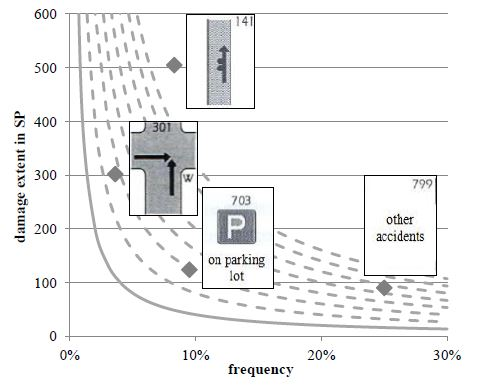
\includegraphics[width=8cm,height=7cm]{figures/Risikoverteilung}
		\caption[Risikoverteilung auf Unfalltypen.]{Risikoverteilung auf Unfalltypen nach \parencite[S. 376]{Gschwendtner.2014}}\label{fig:Risikoverteilung}
	\end{figure}
\end{savenotes}

Häufig werden kleinere Unfälle, wie bereits schon erwähnt, gar nicht von der Polizei aufgenommen. Um die Bewertung für die vorhandenen Daten übernehmen zu könne müsste daher neben der Häufigkeit eine andere Bewertungsmöglichkeit gewählt werden. Anstelle der Schadenspunkte wäre eine Unterteilung der Unfallschwere in fünf Stufen (Kleinunfall, schwerer Sachschaden, leicht Verletzt, schwer Verletzt, getötet) denkbar.

\subsection{Relatives Risiko}
\Textcite[S. 112f]{Grundl.2005} erläutert in seiner Arbeit die Berechnung des Relativen Risikos. Dieses kann verwendet werden, um Auswirkungen bestimmter Risikovariablen wie z.B. Fehler, Verhaltensweisen oder Eigenschaften auf die Entstehung von Unfällen zu beschreiben. Er unterscheidet bei der Berechnung zwischen Verursacher und Beteiligter. Das Relativer Risiko berechnet sich aus dem Quotienten der Unfallverursachungsrate bei Verursachern und der Unfallverursachungsrate bei Beteiligten. %Evtl. direkt als Formel darstellen?
Des weiteren wird bei der Berechnung berücksichtigt, ob ein bestimmter Risikofaktor (z.B. Sonnenblendung) zum Unfallzeitpunkt auftrat. Der Risikofaktor bildet dabei die unabhängige Variable, der Faktor der Unfallverursachung dagegen die abhängige. Zur besseren Veranschaulichung dient die Vier-Felder-Tafel in Abbildung \ref{fig:Relatives Risiko}. 

\begin{savenotes}
	\begin{figure}[H]
		\centering
		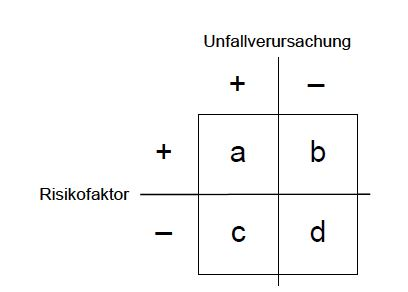
\includegraphics[width=7cm,height=5cm]{figures/Relatives_Risiko}
		\caption[Vier-Felder-Tafel zur Veranschaulichung der Berechnung des Relativen Risikos]{Vier-Felder-Tafel zur Veranschaulichung der Berechnung des Relativen Risikos \parencite[S. 113]{Grundl.2005}}\label{fig:Relatives Risiko}
	\end{figure}
\end{savenotes}

Felder die mit einem \enquote{+} gekennzeichnet sind haben eine positive Variablenausprägung, es handelt sich beim Fahrer z.B. um einen Unfallverursacher bzw. ein Risikofaktor trat zum Unfallzeitpunkt auf. Ein \enquote{-} bedeutet, dass eine Variablenausprägung negativ ist. Das Relative Risiko berechnet sich dann folgendermaßen:

\begin{equation}
	Relatives Risiko = \dfrac{a}{a+b}:\dfrac{c}{c+d}
\end{equation}

Der Wertebereich kann dabei von 0 bis unendlich reichen. Ein Wert über 1 gibt eine Erhöhung des Risikos, ein Wert unter 1 eine Reduzierung an. Hierbei muss berücksichtigt werden, dass die Genauigkeit von der Stichprobengröße abhängig ist. Je mehr Daten vorliegen, desto genauer kann das Relative Risiko berechnet werden.

\subsection{Risikograph}\label{subsection:Risikograph}
\Textcite[S. 50f]{Hillenbrand.2012} stellt den Risikograph nach DIN V 19250 vor. Die DIN V 19250 wurde zwar 2004 zurückgezogen, da sie Teilweise nicht mit der DIN EN 61508 übereinstimmt, der Graph soll hier jedoch trotzdem erläutert werden. Da er bei Bewertungen von Situationen und Unfälle durchaus nützlich sein kann.

Um Systeme so zu entwickeln, dass Gefährdungen möglichst vermieden werden, werden Systeme in Kategorien eingeordnet. Jede Kategorie bezieht sich auf ein qualitativ oder quantitativ festgelegtes Risikointervall und ist direkt mit Anforderungen an die Sicherheit des Systems verbunden. Das Risiko wird hier als Paar aus Ereignishäufigkeit H und Schadensausmaß S angenommen. Die Häufigkeit H wird weiter unterteilt in Aufenthaltsdauer A, Gefahrenabwendung G und Wahrscheinlichkeit des unerwünschten Ereignisses W. Der Risikograph in Abbildung \ref{fig:Risikograph} dient der Kategorisierung von Systemen. Die Einordnung in die Kategorien a bis h erfolgt durch die Betrachtung der Variablen S, A, G und W in Tabelle \ref{tab:Kategorisierung nach DIN V 19250}. Hierbei gilt, je höher der Ordnungswert, desto höher ist das mit dem System verbundene Risiko.

\begin{savenotes}
	\begin{figure}[H]
		\centering
		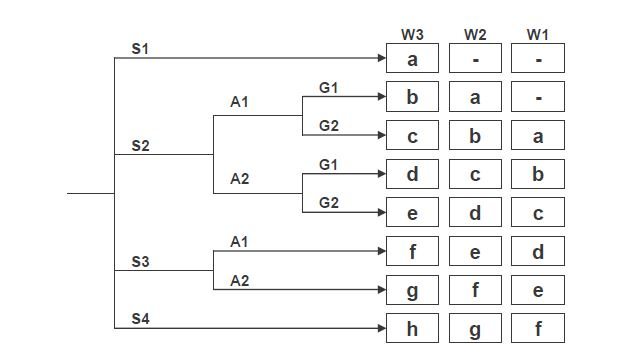
\includegraphics[width=9cm,height=6cm]{figures/Risikograph}
		\caption[Risikograph nach DIN V 1925]{Risikograph nach DIN V 19250 \parencite[S. 51]{Hillenbrand.2012}}\label{fig:Risikograph}
	\end{figure}
\end{savenotes}

\begin{table}[htpb]
	\scriptsize
	\caption[Kategorisierung nach DIN V 19250]{Kategorisierung nach DIN V 19250 \parencite[S. 52]{Hillenbrand.2012}}\label{tab:Kategorisierung nach DIN V 19250}
	\centering
	\begin{tabular}{l l p{7cm}}
		\toprule
		Schadensausmaß & S1 & Leichte Verletzung einer Person, kleinere schädliche Umwelteinflüsse\\
		 & S2 & Schwere irreversible Verletzungen einer oder mehrerer Personen oder Tod einer Person; vorübergehende, größere, schädliche Umwelteinflüsse\\
		 & S3 & Tod mehrerer Personen; lang andauernde, größere, schädliche Umwelteinflüsse\\
		 & S4 & Katastrophale Auswirkungen, sehr viele Tote\\
		\midrule
		Aufenthaltsdauer & A1 & selten bis öfter\\
		 & A2 & häufig bis dauernd\\
		 \midrule
		 Gefahrenabwendung & G1 & möglich unter bestimmten Bedingungen\\
		 & G2 & kaum möglich\\
		 \midrule
		 Eintrittswahrscheinlichkeit & W1 & sehr gering\\
		 & W2 & gering\\
		 & W3 & relativ hoch\\
		\bottomrule
	\end{tabular}
\end{table}

% Auf S. 53 wird in einer Tabelle dargestellt, welchen SIL die Buchstaben a bis h des Risikographs entsprechen. Brauch ich das hier?

\subsection{Gefährdungs- und Risikoanalyse}
\enquote{Teil 3: Konzeptphase der ISO 26262} enthält eine Gefährdungs- und Risikoanalyse. Diese ist auf den Automobilbereich zugeschnitten und klassifiziert Gefährdungen anhand der in Tabelle \ref{tab:Kategorisierung nach ISO 26262} dargestellten Kriterien.

\begin{table}[htpb]
	\scriptsize
	\caption[Klassifizierung der Gefährdungen nach ISO 26262]{Klassifizierung der Gefährdungen nach ISO 26262 \parencite[S. 95]{Hillenbrand.2012}}\label{tab:Kategorisierung nach ISO 26262}
	\centering
	\begin{tabular}{l l p{7cm}}
		\toprule
		Schwere eine möglichen Schadens & S0 & Keine Verletzungen\\
		& S1 & Leichte bis mittlere Verletzungen\\
		& S2 & Schwere Verletzungen, Überleben wahrscheinlich\\
		& S3 & Lebensgefährliche Verletzungen, Überleben unwahrscheinlich\\
		\midrule
		Häufigkeit der Fahrsituation & E0 & Unvorstellbar\\
		& E1 & Sehr niedrige Wahrscheinlichkeit\\
		& E2 & Niedrige Wahrscheinlichkeit\\
		& E3 & Mittlere Wahrscheinlichkeit\\
		& E4 & Hohe Wahrscheinlichkeit\\
		\midrule
		Beherrschbarkeit durch den Fahrer & C0 & Im allgemeinen Beherrschbar\\
		& C1 & Einfach beherrschbar\\
		& C2 & Normalerweise beherrschbar\\
		& C3 & Schwierig oder nicht beherrschbar\\
		\bottomrule
	\end{tabular}
\end{table}

Die Klassifizierungen in Tabelle \ref{tab:Kategorisierung nach ISO 26262} dienen der Gefährdungsbestimmung nach Abbildung \ref{fig:ISO 26262}. Während QM nur einfache Maßnahmen des Qualitätsmanagements betrifft erfordern die Werte A bis D spezielle Maßnahmen. Die Werte werden auch als \acp{ASIL} bezeichnet und stellen Klassen zur Spezifizierung der notwendigen Sicherheitsanforderungen des Systems, um ein akzeptables Risiko zu erzielen, dar. Die höchste Klasse ist \acs{ASIL} D, sie erfordert die effektivsten Maßnahmen \parencite[S.94ff]{Hillenbrand.2012}.

\begin{savenotes}
	\begin{figure}[H]
		\centering
		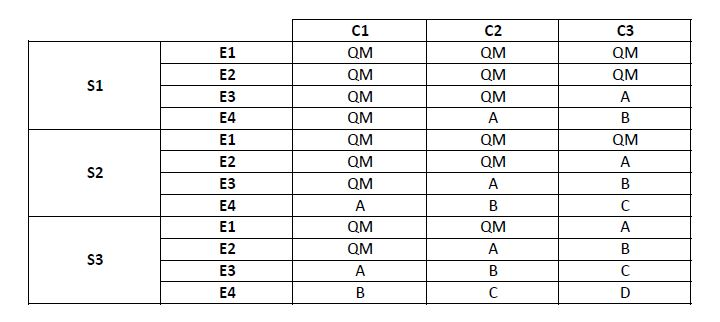
\includegraphics[width=12cm,height=5cm]{figures/ISO_26262}
		\caption[ASIL Bestimmung nach ISO 26262]{ASIL Bestimmung nach ISO 26262 \parencite[S. 96]{Hillenbrand.2012}}\label{fig:ISO 26262}
	\end{figure}
\end{savenotes}

\subsection{Konfliktschweregrade und Komplexität von Verkehrssituationen}
Neben der reinen Unfallanalyse ist es möglich verschiedene Situationen zu betrachten, die zu Konflikten führen, aus denen sich jedoch nicht immer ein Unfall ereignet. \Textcite[S. 28]{Erke.1978} definiert vier Konfliktschweregrade anhand der Zeit die dem Fahrer zur Verfügung steht um auf eine Situation zu reagieren:

\begin{itemize}
	\item Schweregrad 1: Der Fahrer hat gerade noch genug Zeit um kritische Fahrmanöver kontrolliert auszuführen. Dabei ist zusätzlich Zeit zur Orientierung und Zeit zum Anzeigen der eigenen Absicht (Blinken) vorhanden. Eine Beispielsituation ist kontrolliertes Bremsen und/oder Ausweichen.
	\item Schweregrad 2: Der Fahrer hat keine Zeit mehr kritische Fahrmanöver kontrolliert durchzuführen. Hierbei kann es sich z.B. um starkes Bremsen und/oder abruptes Ausweichen handeln. Es ist gerade noch genug Zeit vorhanden, die Situation der anderen Verkehrsteilnehmer zu berücksichtigen, die Zeit reicht allerdings nicht aus um seine Absicht anzuzeigen. Es kann zu Folgekonflikten mit geringem Schweregrad kommen.
	\item Schweregrad 4: Der Fahrer kann nur durch eine sehr schnelle Reaktion, z.B. Notbremsung, eine Kollision verhindern (Beinahe-Unfall). Er ist dabei nicht mehr in der Lage die Situation der anderen Verkehrsteilnehmer zu berücksichtigen. Unter Umständen kommt es zu Folgekonflikten des Schweregrades 2.
	\item Schweregrad 4: Der Fahrer hat nicht mehr genügend Zeit, um auf den Konfliktgegner zu reagieren. Es kommt zur Kollision.
\end{itemize}

Die genannten Schweregrade befassen sich nur mit der Zeit die bleibt um unfallvermeidende Fahrmanöver durchzuführen. Es werden keine Beispiele genannt, wann bzw. wo es zu Situationen mit den unterschiedlichen Schweregraden kommen kann. \Textcite[S. 33f]{Meitinger.2008} dagegen definiert die Komplexität von verschiedenen Verkehrssituationen in drei Kategorien:

\begin{itemize}
	\item Komplexe Situation: Mehrspurige Fahrbahn in der Kreuzung oder hohe Verkehrsdichte oder hohe Anforderungen an die Spurführung oder unübersichtliche Kreuzung
	\item Mittel komplexe Situation: Größere Kreuzung (z.B. an einer Bundesstraße) aber kein Hinweis auf höhere Verkehrsdichte oder ungünstige Umweltbedingungen
	\item Einfache Situation: Kleine übersichtlich Kreuzung
\end{itemize}

Während die Bewertung der Verkehrssituationen bei der Unfallauswertung berücksichtigt werden kann, ist die Aufteilung der Konflikte in verschiedene Schweregrade nicht hilfreich. Es kam bereits zu einem Unfall es lag also allen Situationen, der Schweregrad 4 zugrunde. Betrachtet man dagegen Fahrsituationen die in einem bestimmten Gebiet auftreten oder markante Knotenpunkte unabhängig von sich bereits ereigneten Unfällen über einen gewissen Zeitraum kann die Unterteilung in Konfliktschweregrade durchaus Sinnvoll sein.


\section{Weiterer Forschungsbedarf}
\enquote{Die amtliche Erfassung von Verkehrsunfällen hat in Deutschland eine hohe Qualität} \parencite[S. 821]{Brilon.2016}. Dies ist darauf zurückzuführen, dass es in den 60er-Jahren gelungen ist ein bundesweites Erfassung- und Klassifizierungssystem weitgehend einheitlich einzuführen. Grundlage lieferte damals eine von von Pfundt entwickelte \enquote{Typisierung der Verkehrsunfälle nach der Art der Unfallentstehung}. Trotz der vermeintlich hohen Qualität liegt die Einführung des Systems nun ungefähr 50 Jahre zurück und müsste überarbeitet werden. Denn manche Teilbereiche werden nicht ausführlich genug erfasst. Auch \Textcite[S. 69]{Burger.1983} erwähnte bereits in seiner Dissertation, dass das Erkennen und Nachweisen von Zusammenhängen zwischen zahlreichen Variablen eines Unfalls eine wesentliche Aufgabe der Unfallforschung darstellt. Um diese Zusammenhänge nachweisen zu können müssen jedoch die verschiedenen Variablen der Unfälle genauestens erfasst werden. Dies ist heute, 35 Jahre später, leider immer noche selten der Fall. Es gibt zwar Projekte, wie \ac{GIDAS}, die sich bemühen Unfalldaten so genau wie möglich zu ermitteln. Doch auch hier werden nur Unfälle genauer erfasst, bei denen es zu einem Personenschaden kam. \Textcite[S. 18]{Gschwendtner.2015} stellt im Verlauf seiner Arbeit ebenfalls fest, dass die Klassifizierung von Unfällen auf Personenschäden ausgerichtet ist. Die offiziellen Statistiken ermöglichen keine Aussagen zu konfliktauslösenden Szenarien, Unfallarten und Unfallursachen die lediglich zu Unfällen mit Sachschäden führen. Zu vielen Unfällen die nur zu Sachschaden führen liegen entweder gar keine oder nur sehr unzureichende Informationen vor. Um alle Umfeldbedingungen für das voll automatisiertes Fahren zu erfassen müssen die Dunkelziffern der nicht erfassten Unfälle weitestgehend reduziert werden. Denn nur so gelingt es ein nahezu vollständiges Bild aller Situationen zu erhalten, die zu Konflikten führen können. Hierfür wäre es möglich die bei den Erhebungen z.B. von \ac{GIDAS} verwendeten Methoden auf Sachschadensunfälle zu übertragen. Zusätzlich müssten wie in Kapitel \ref{Urabane Fahrsituationen mit geringen Geschwindigkeiten} bereits erwähnt die Unfalltypen und Unfallarten so angepasst werden, dass bei der Aufnahme von Unfällen mit geringem Schaden aussagekräftige Erkenntnisse entstehen.
  
Ein weiterer negativer Punkt ist, dass häufig von Unfällen die sich bereits ereignet haben auf mögliche Konfliktpunkte geschlossen wird. Besser wäre es, Konfliktsituationen zu analysieren. Denn Konflikte beschreiben den Ablauf des Verkehrs differenzierter als die Unfälle \parencite[S. 13]{Erke.1978}. Trotzdem findet sich wenig Literatur zur Auswertung von Verkehrskonflikten. Die Beobachtung des gesamten Verkehrsablaufs über einen längeren Zeitraum wäre zu Zeitaufwendig. Deshalb werden nur die Situationen bzw. Bereiche analysiert, bei denen es bereits zu Unfällen kam. Hier werden dann zum Teil auch Verkehrsbeobachtungen durchgeführt um die Konfliktsituationen besser analysieren zu können.
